\chapter{GRÁFICOS DOS SCORES GERADOS PELO COMITÊ DE REDES NEURAIS}

\section{Score da onda gravitacional GW151012}
\begin{figure*}[ht]
     \subfigure[Score gerado para o laboratório H]{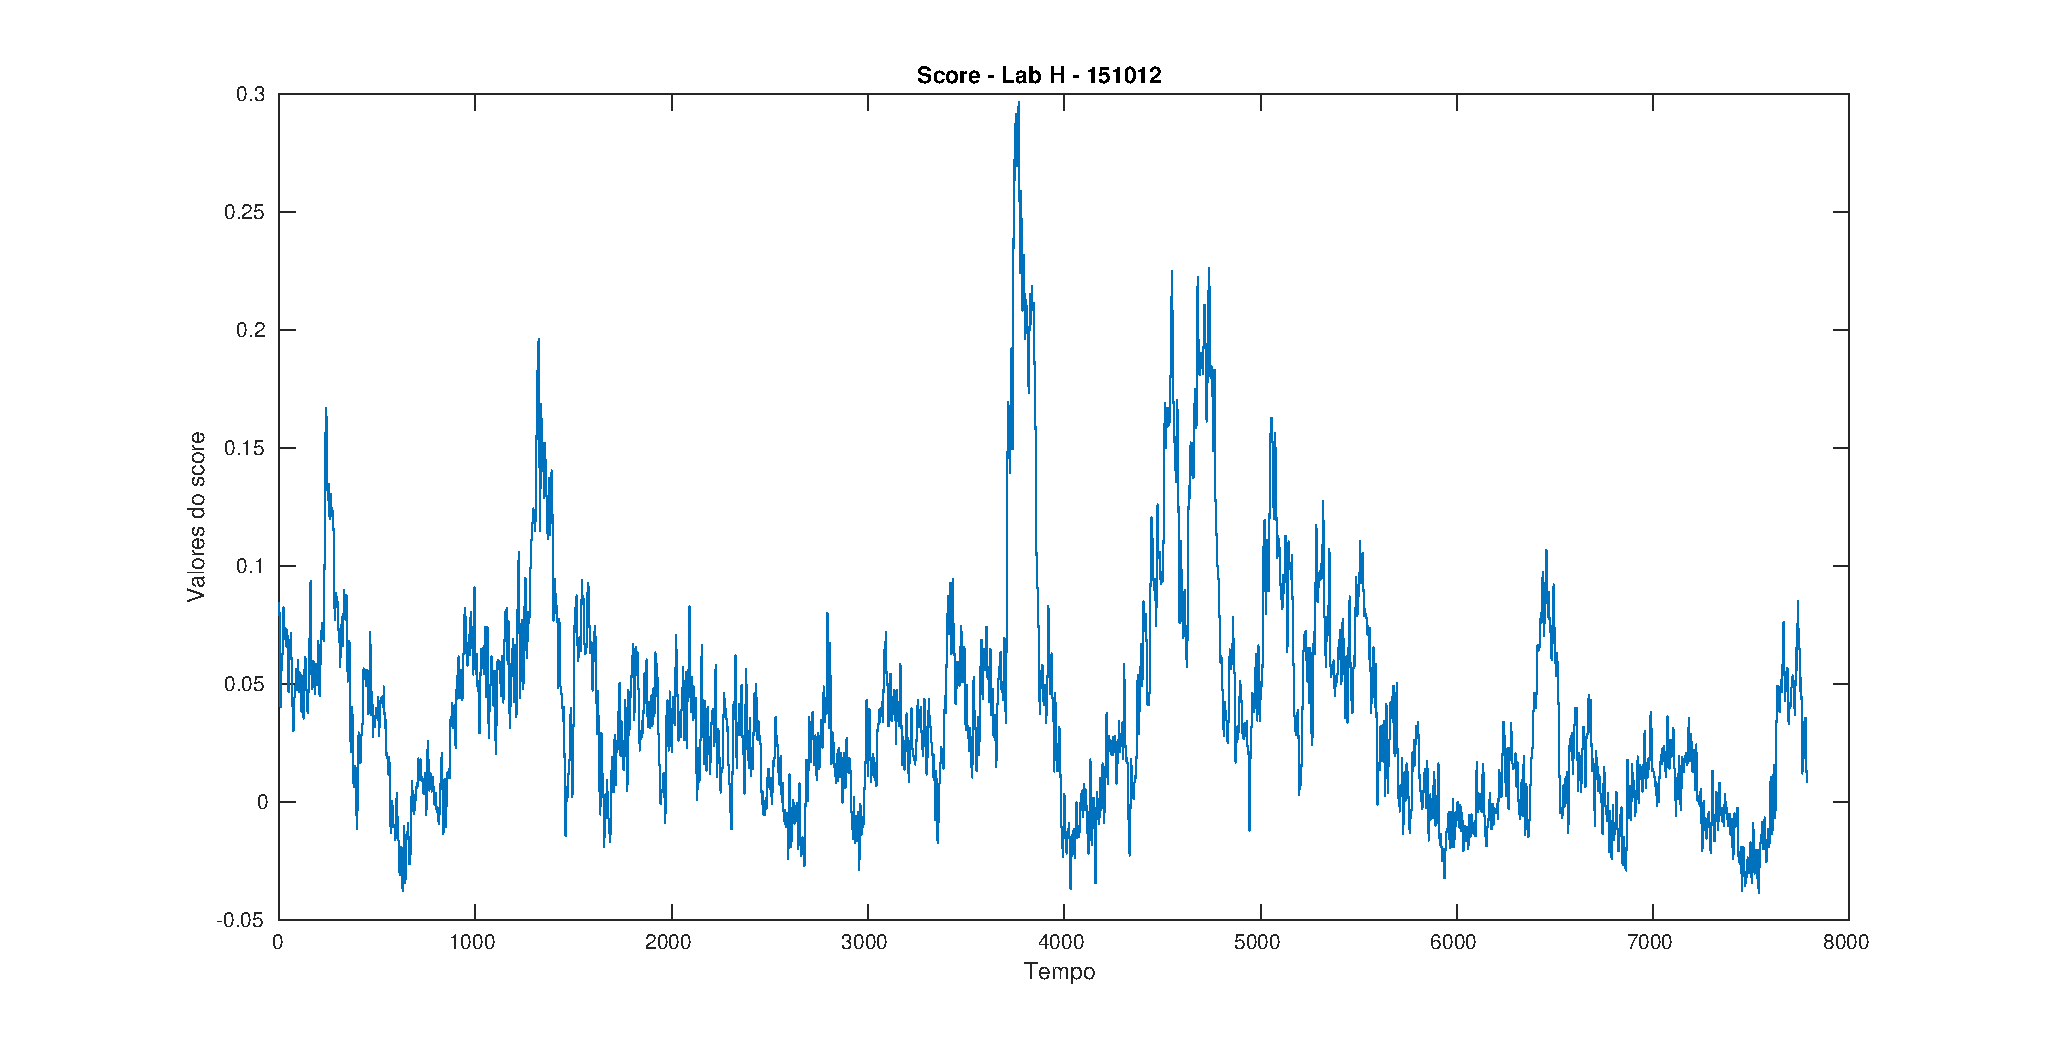
\includegraphics[width=0.5\textwidth]{figuras/GW151012_LabH.eps}}
     \subfigure[Score gerado para o laboratório L]{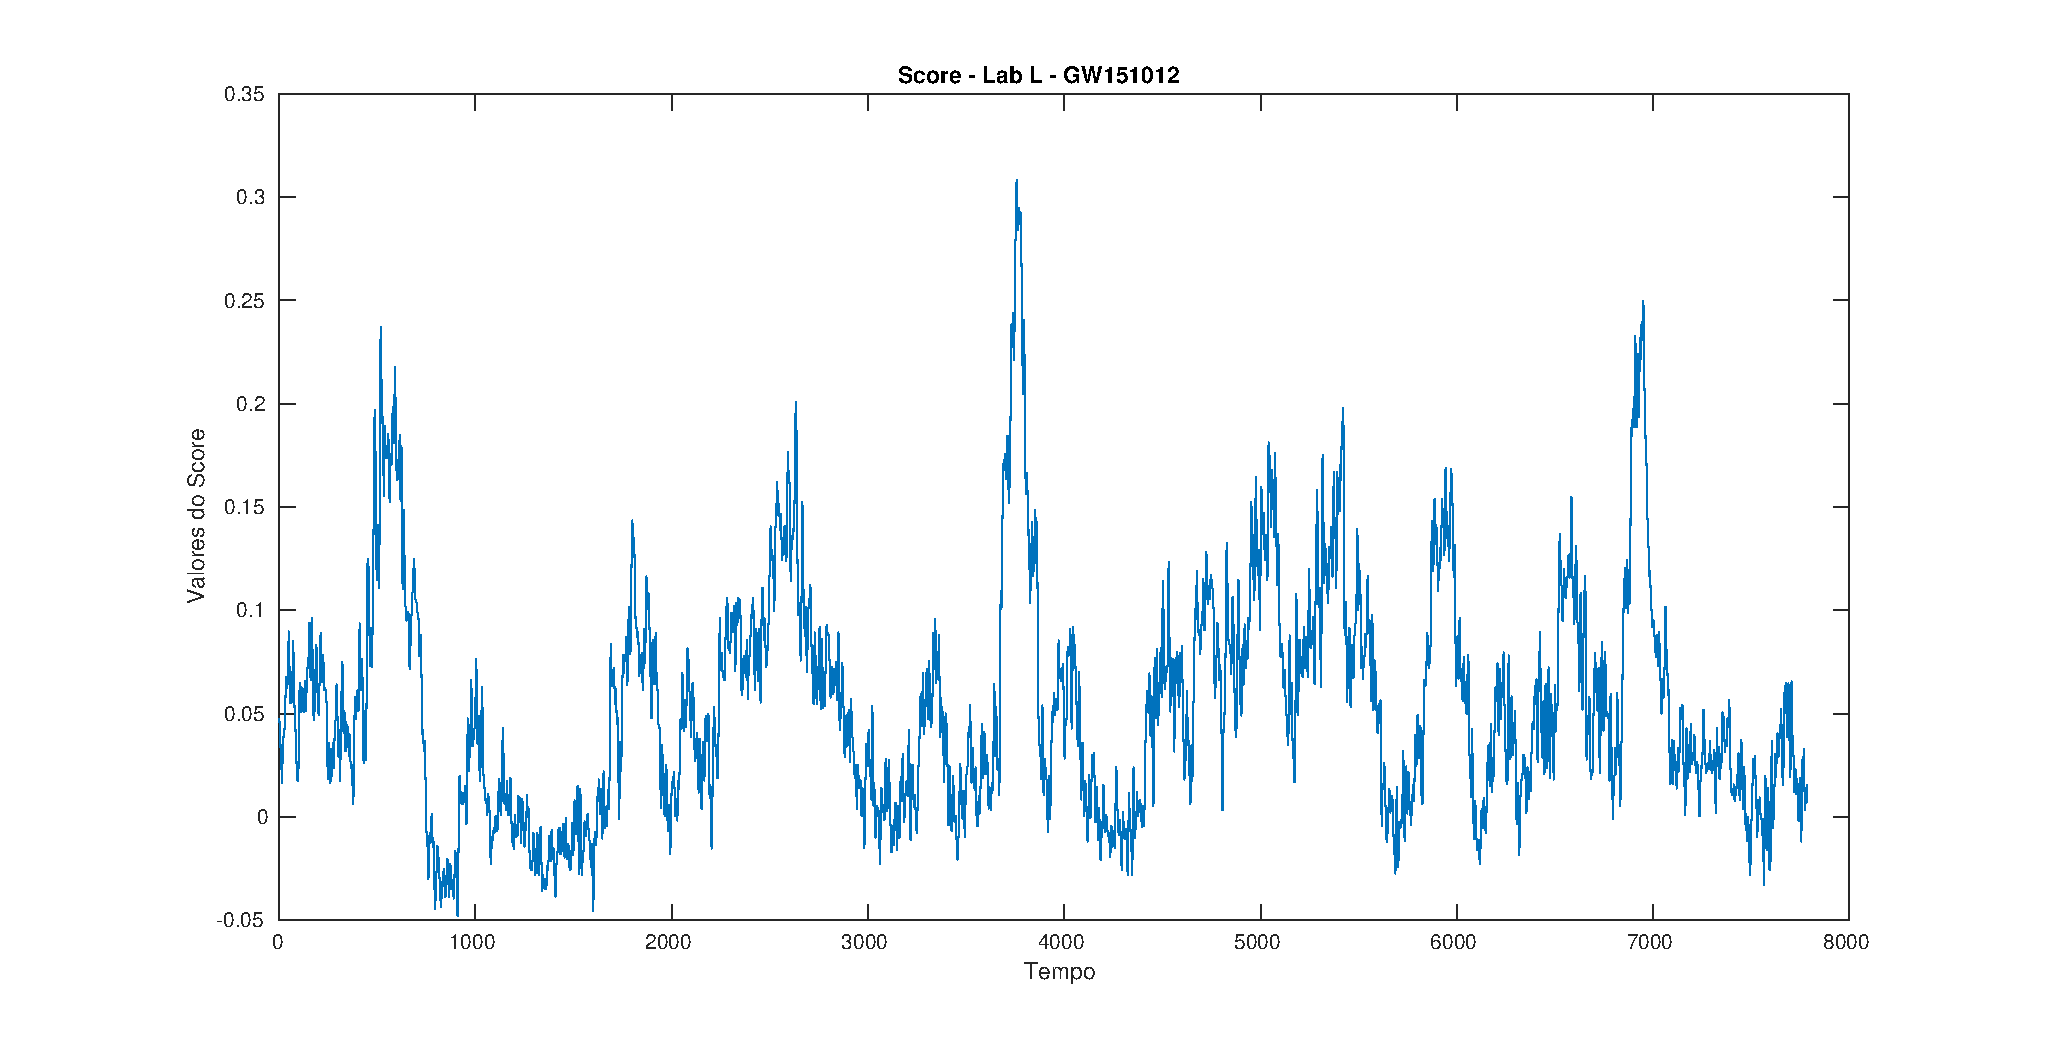
\includegraphics[width=0.5\textwidth]{figuras/GW151012_LabL.eps}}
     \subfigure[Coincidência entre os dois scores]{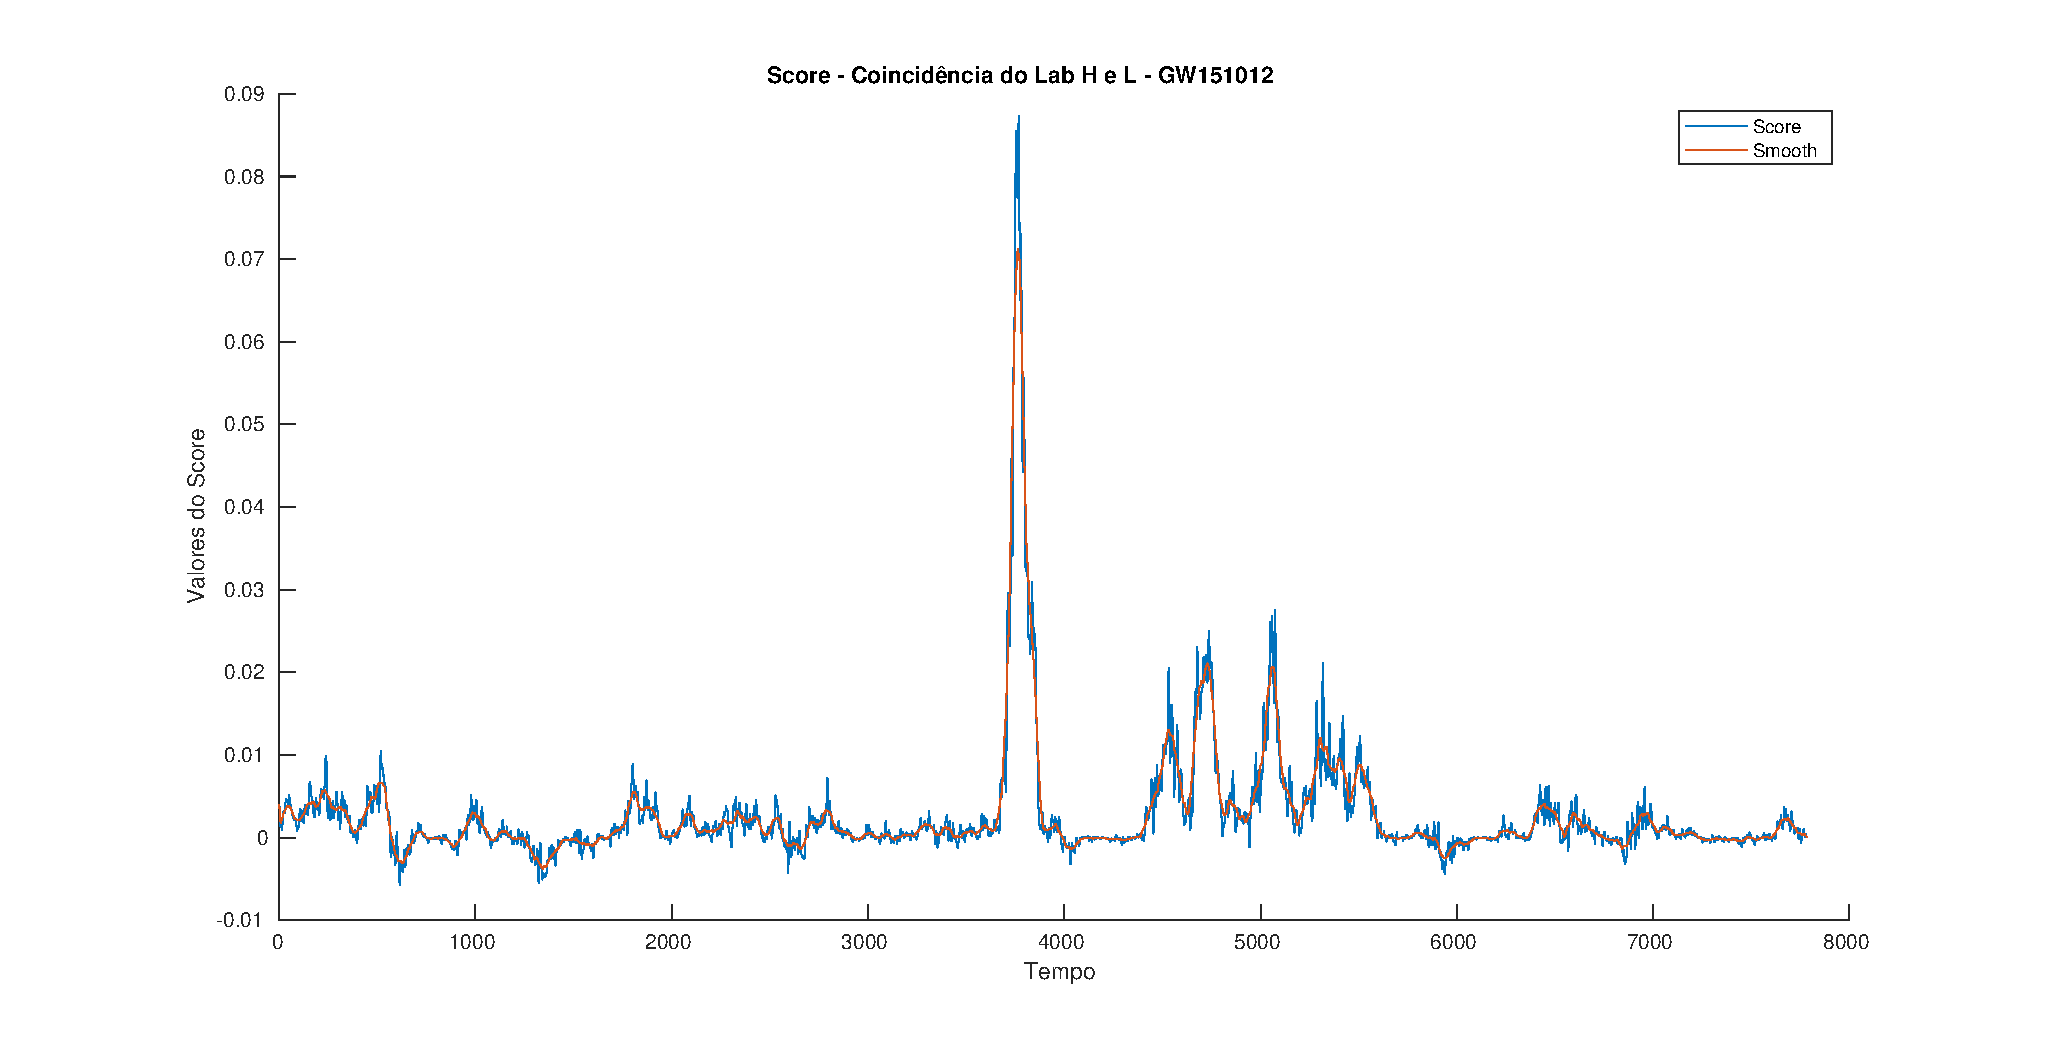
\includegraphics[width=1.0\textwidth]{figuras/GW151012_LabHL.eps}}
     \caption{Score da onda gravitacional GW151012}
 \end{figure*}
 
\section{Score da onda gravitacional GW151226}
\begin{figure}[H]
     \subfigure[Score gerado para o laboratório H]{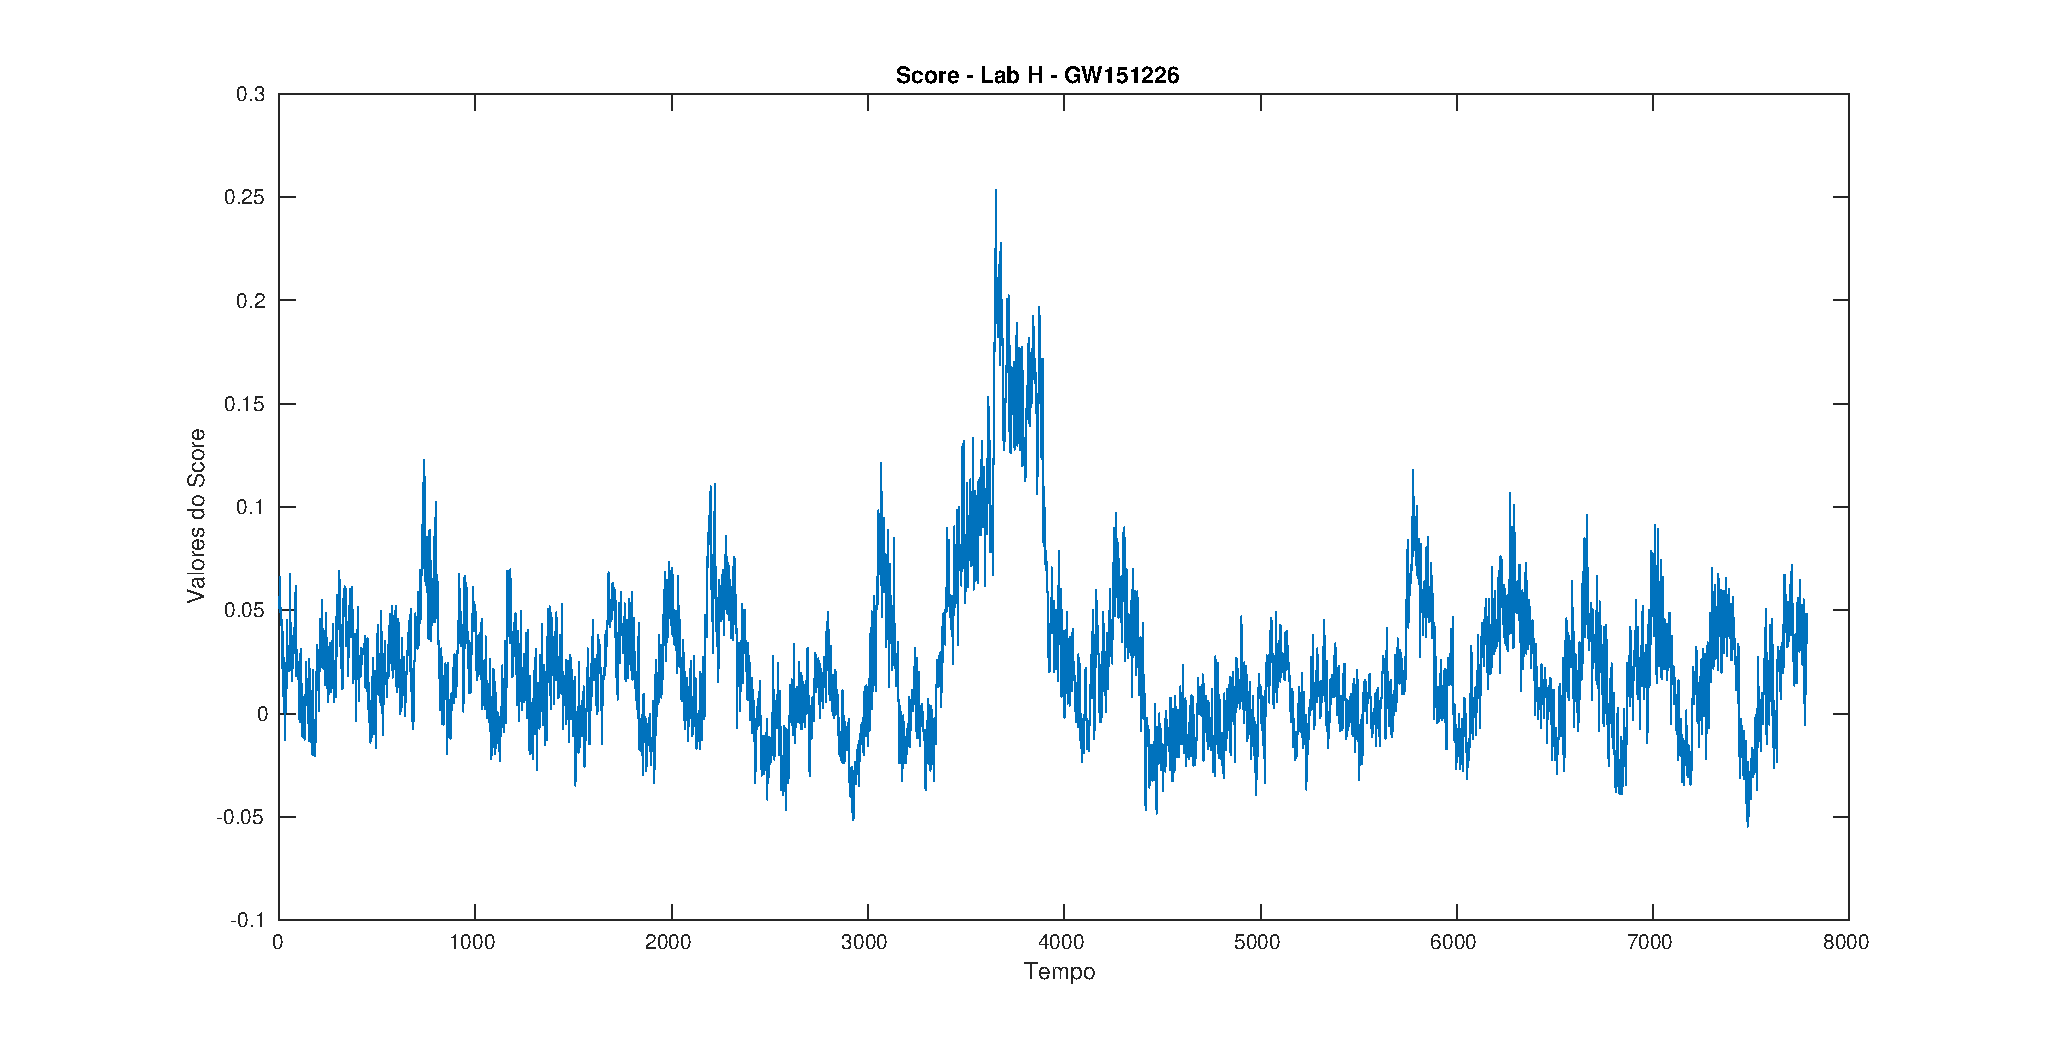
\includegraphics[width=0.5\textwidth]{figuras/GW151226_LabH.eps}}
     \subfigure[Score gerado para o laboratório L]{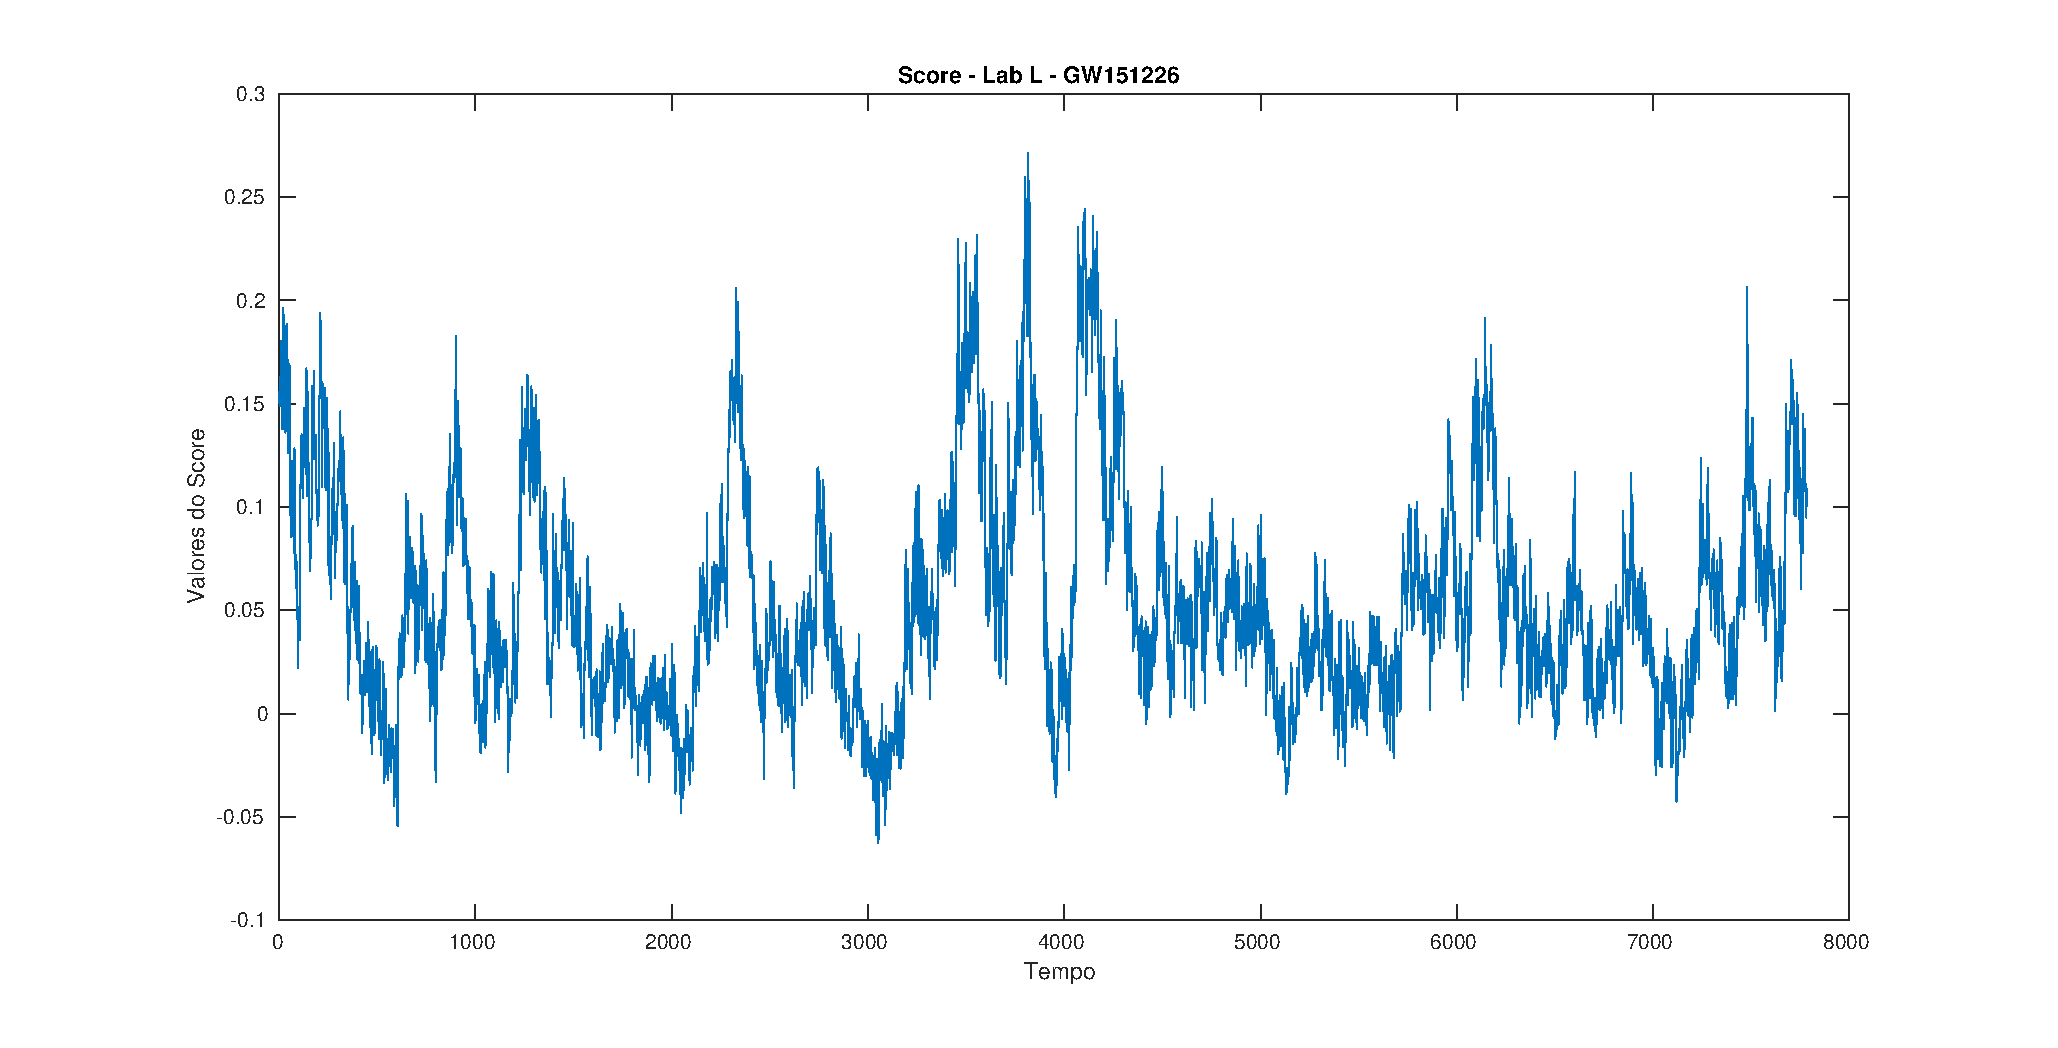
\includegraphics[width=0.5\textwidth]{figuras/GW151226_LabL.eps}}
     \subfigure[Coincidência entre os dois scores]{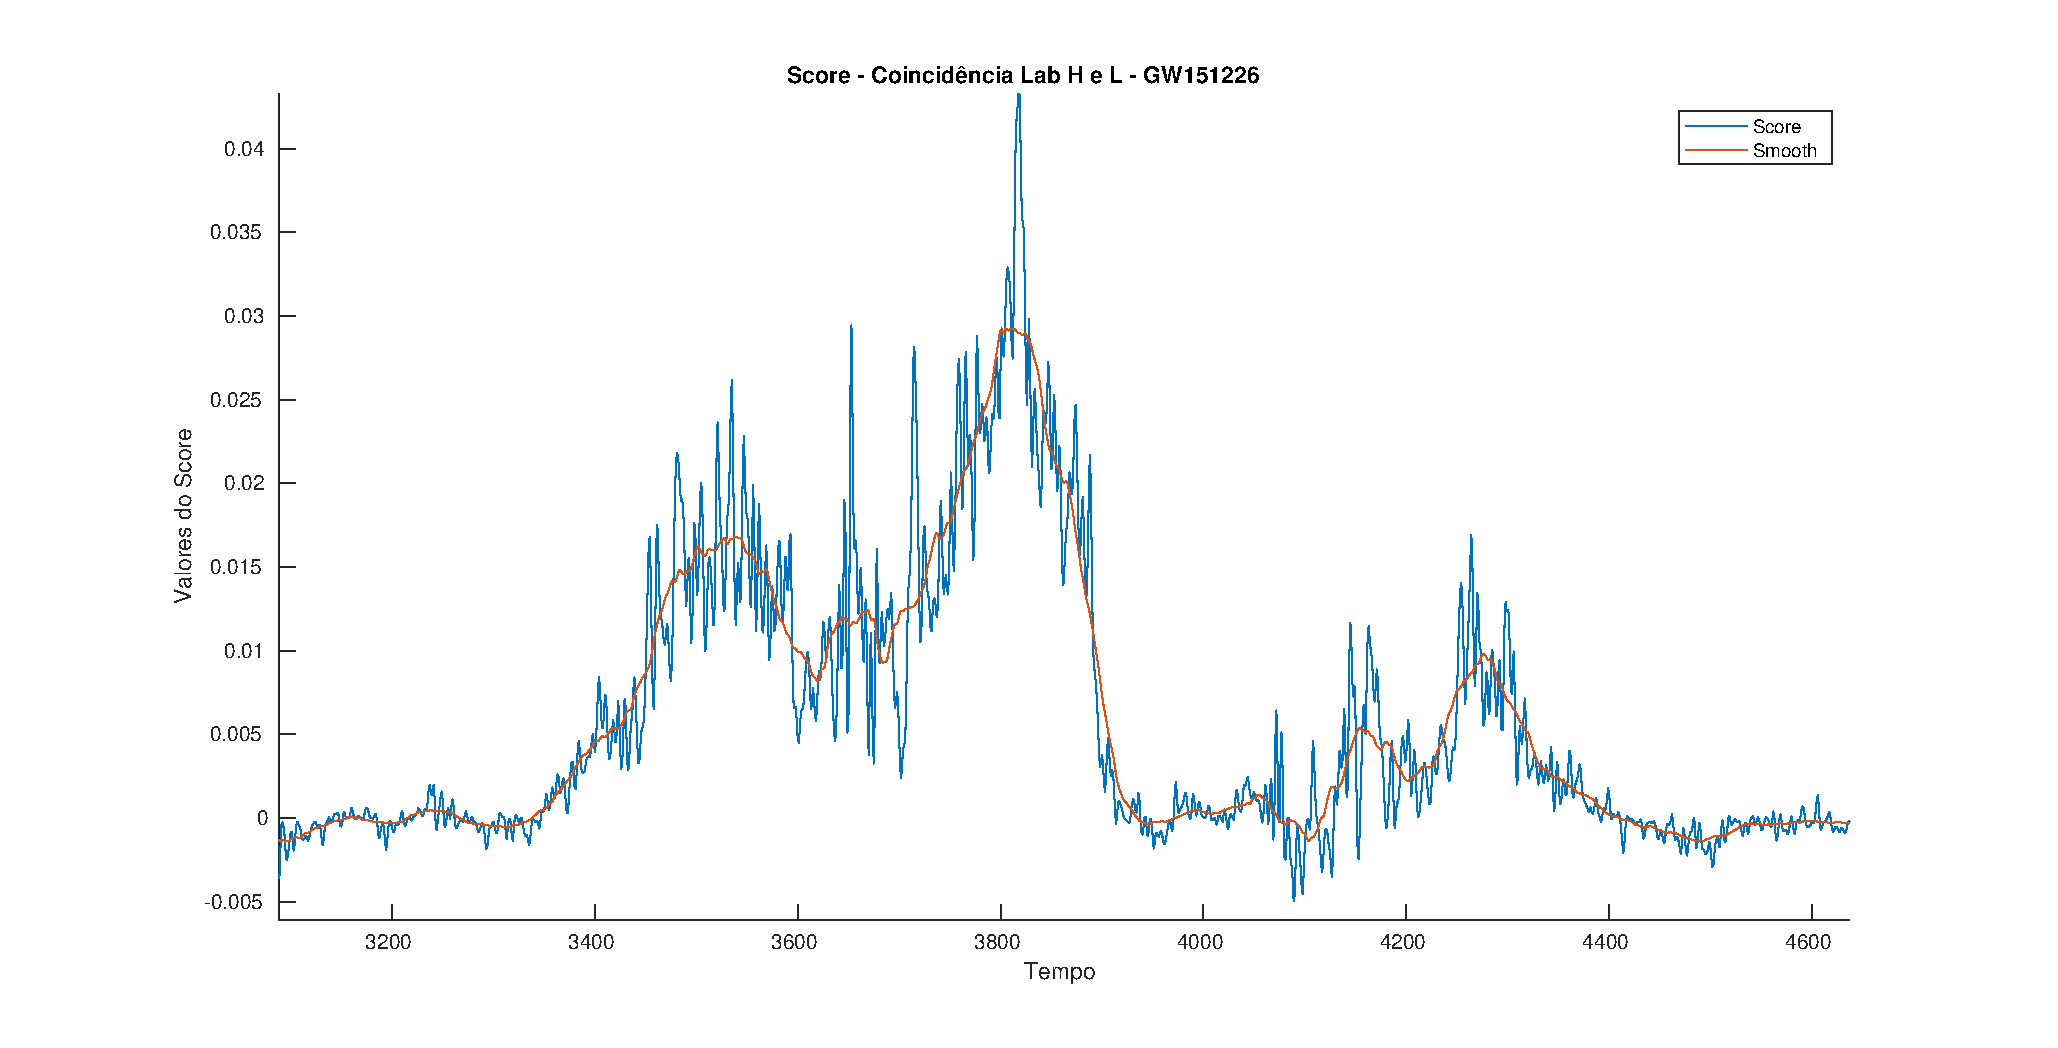
\includegraphics[width=1.0\textwidth]{figuras/GW151226_LabHL.eps}}
     \caption{Score da onda gravitacional GW151226}
 \end{figure}
 
\section{Score da onda gravitacional GW170104}
\begin{figure}[H]
     \subfigure[Score gerado para o laboratório H]{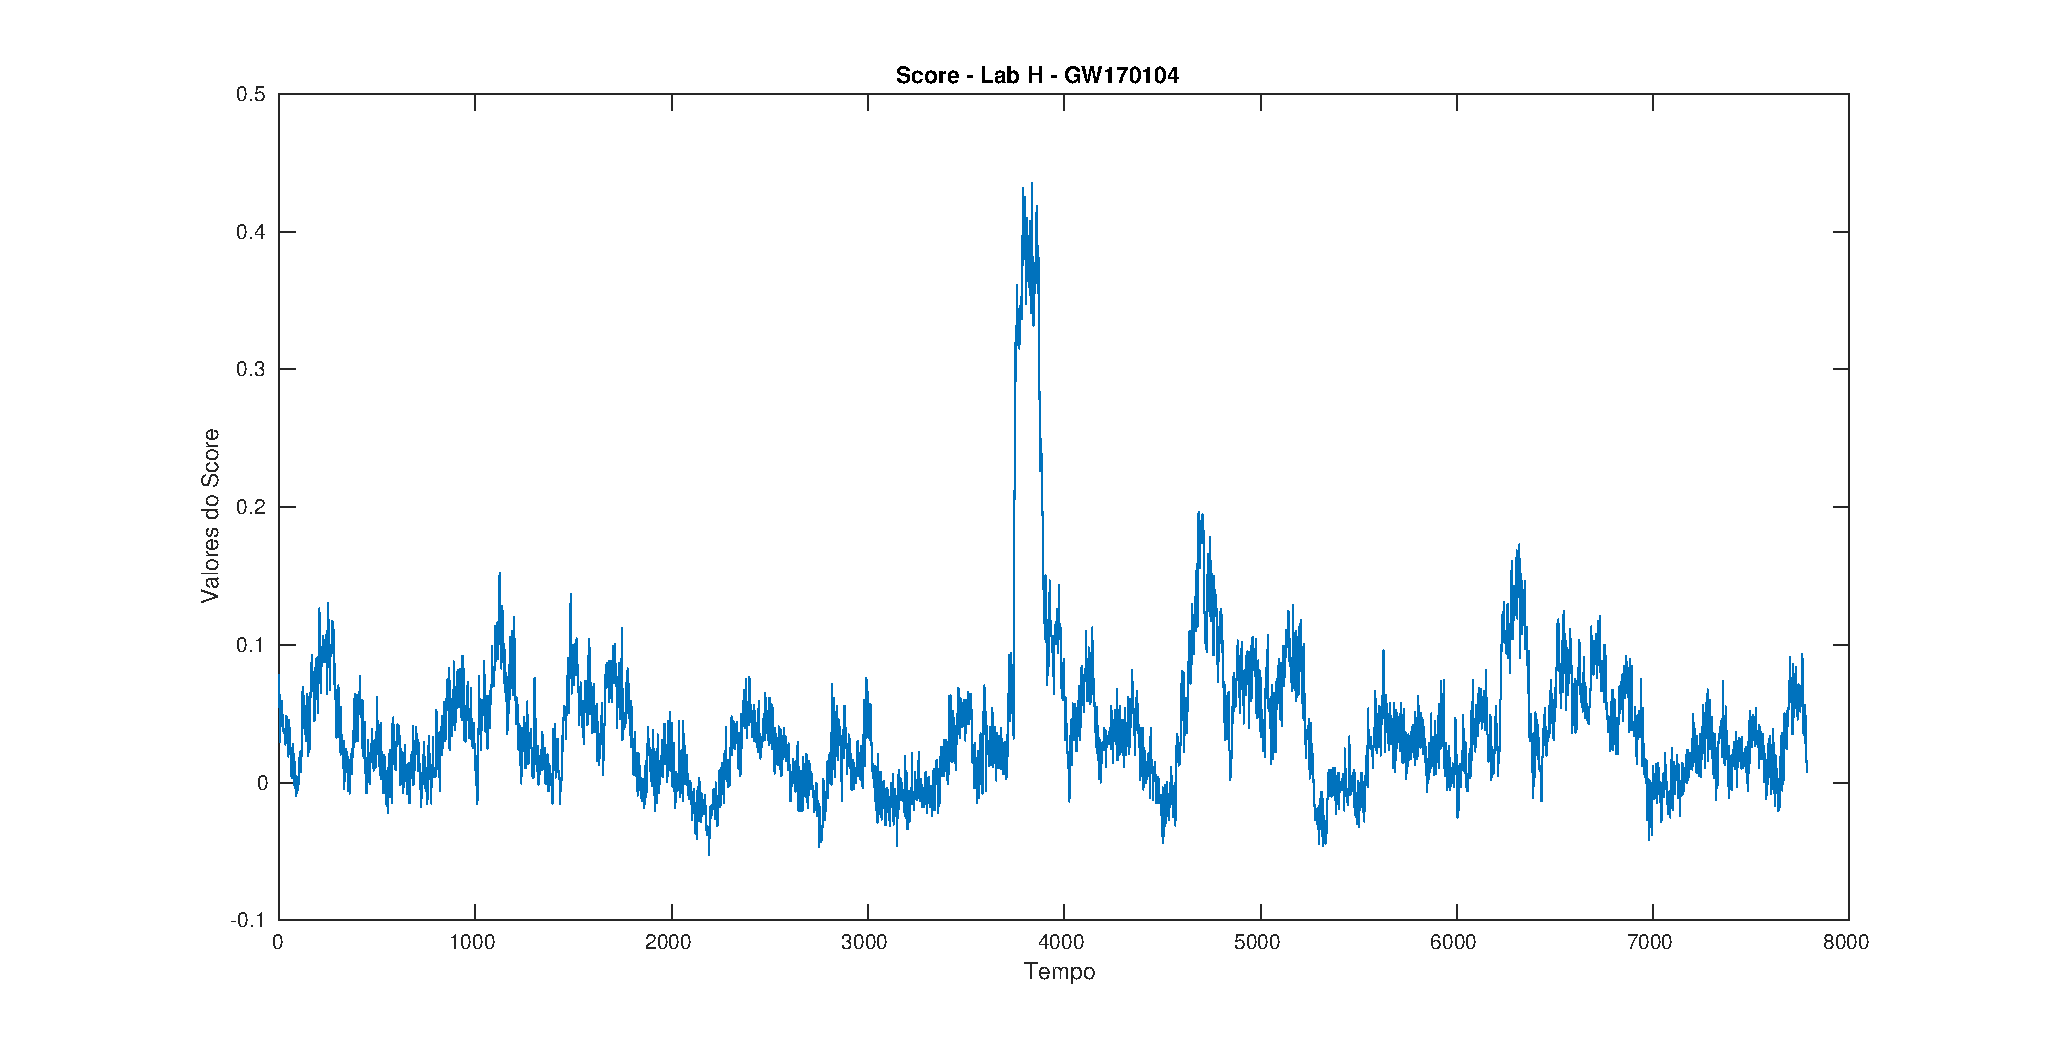
\includegraphics[width=0.5\textwidth]{figuras/GW170104_LabH.eps}}
     \subfigure[Score gerado para o laboratório L]{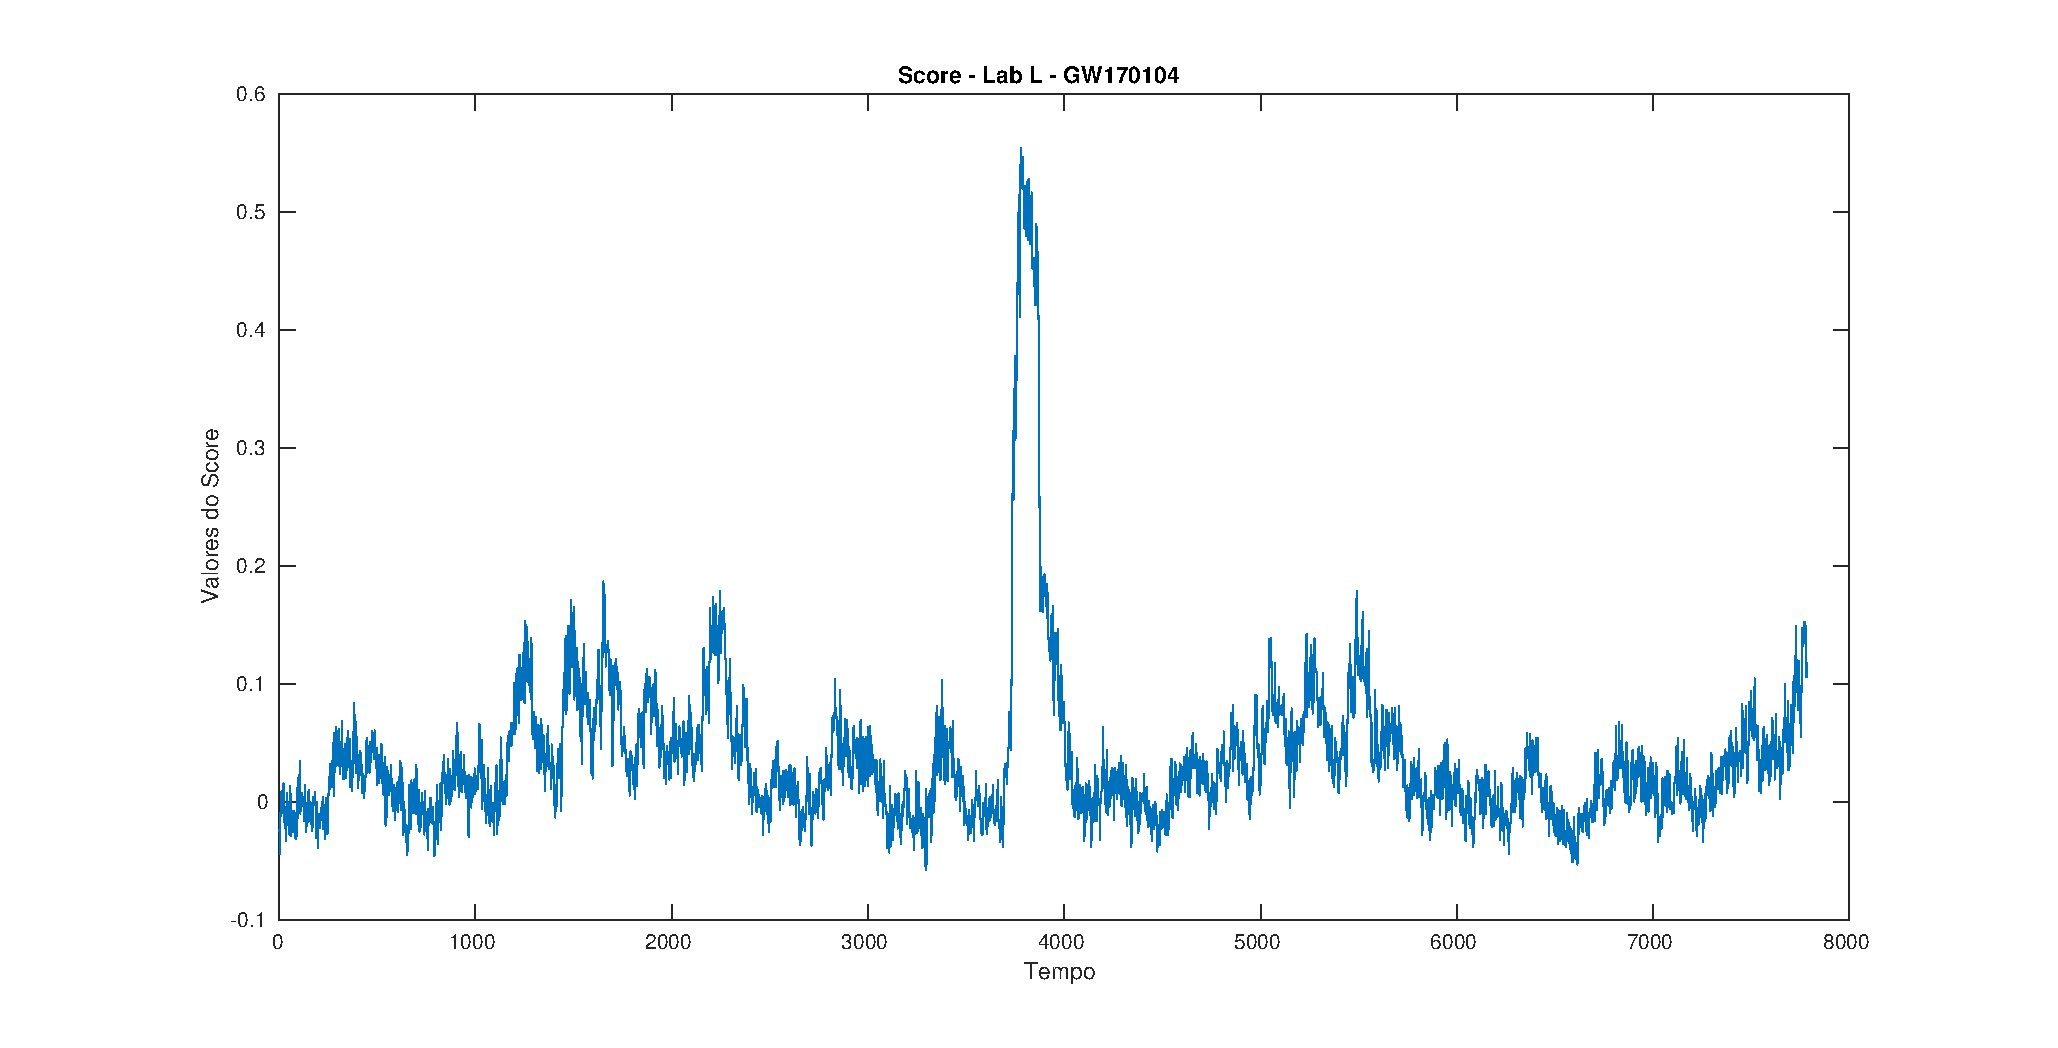
\includegraphics[width=0.5\textwidth]{figuras/GW170104_LabL.eps}}
     \subfigure[Coincidência entre os dois scores]{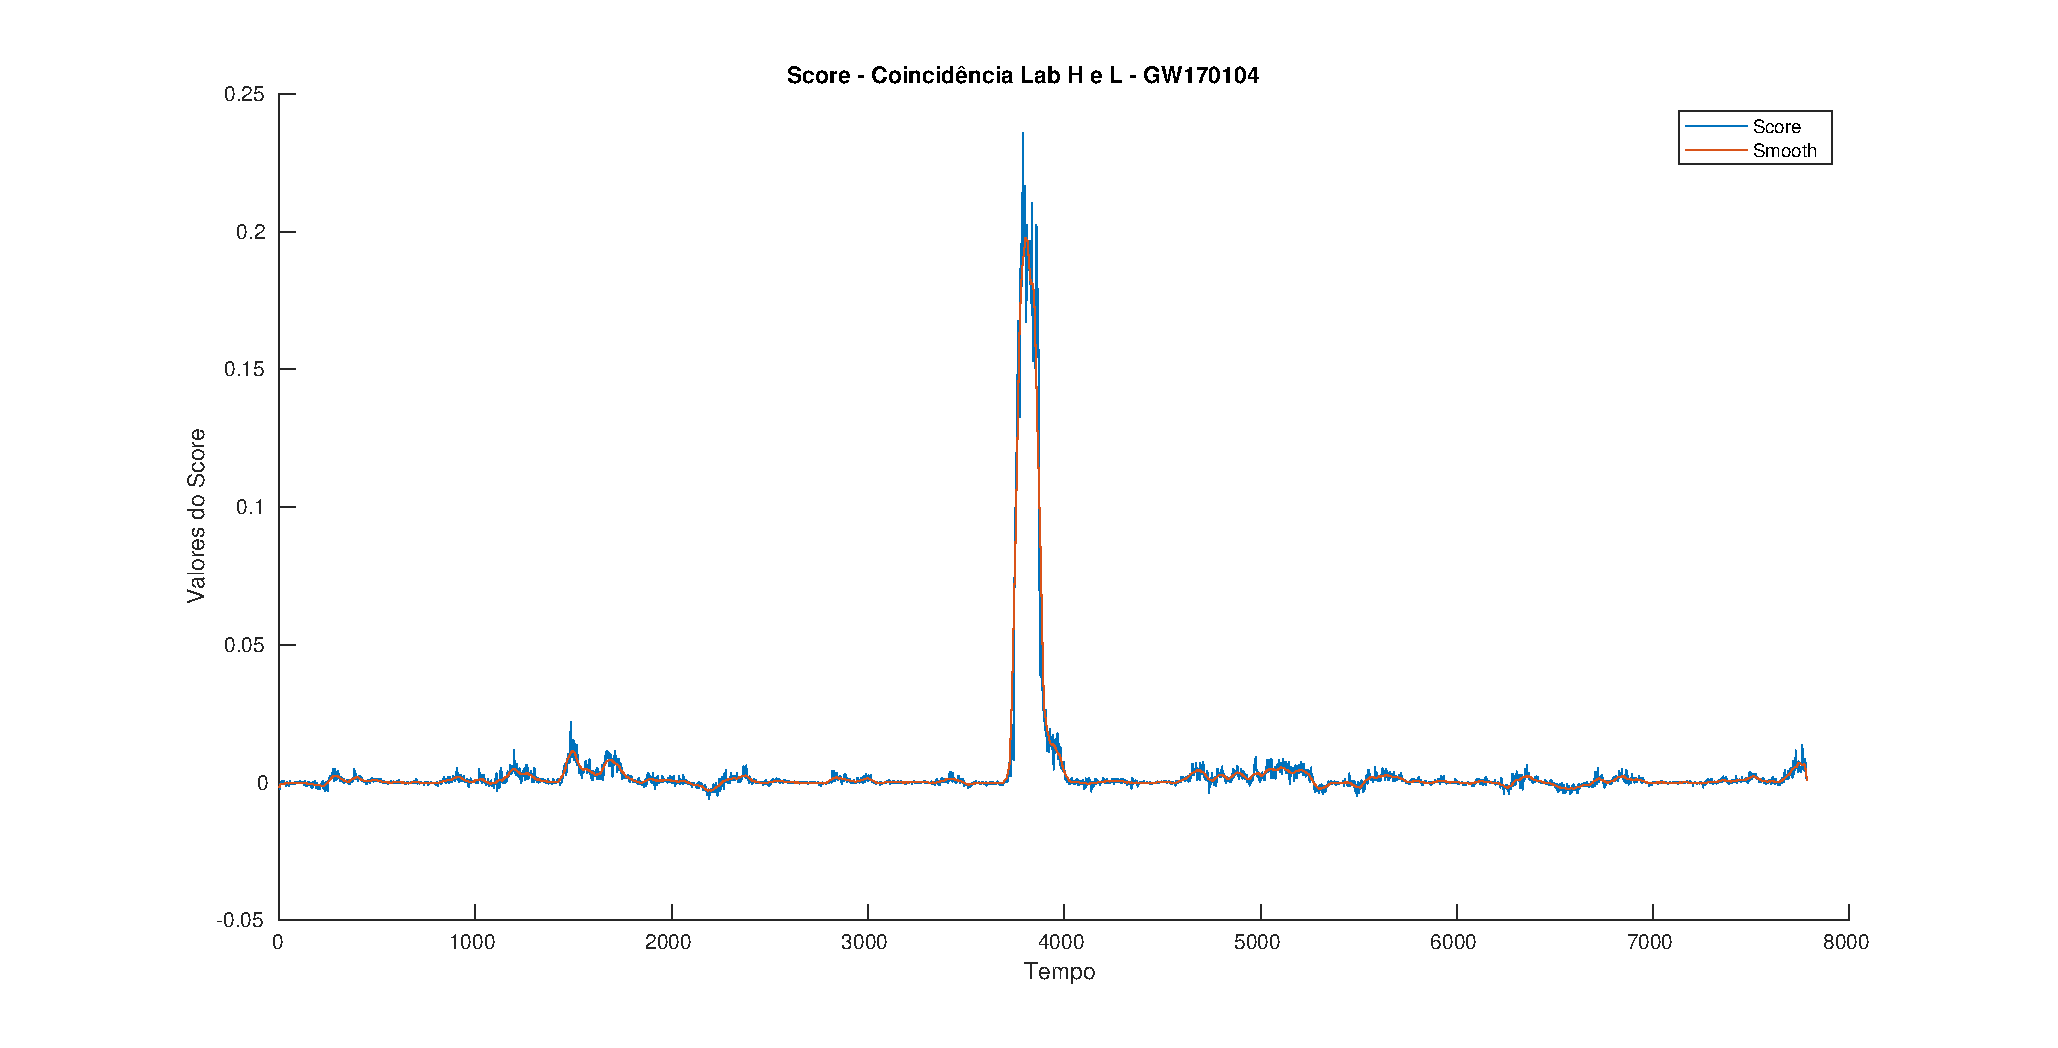
\includegraphics[width=1.0\textwidth]{figuras/GW170104_LabHL.eps}}
     \caption{Score da onda gravitacional GW170104}
 \end{figure}

\section{Score da onda gravitacional GW170608}
\begin{figure}[H]
     \subfigure[Score gerado para o laboratório H]{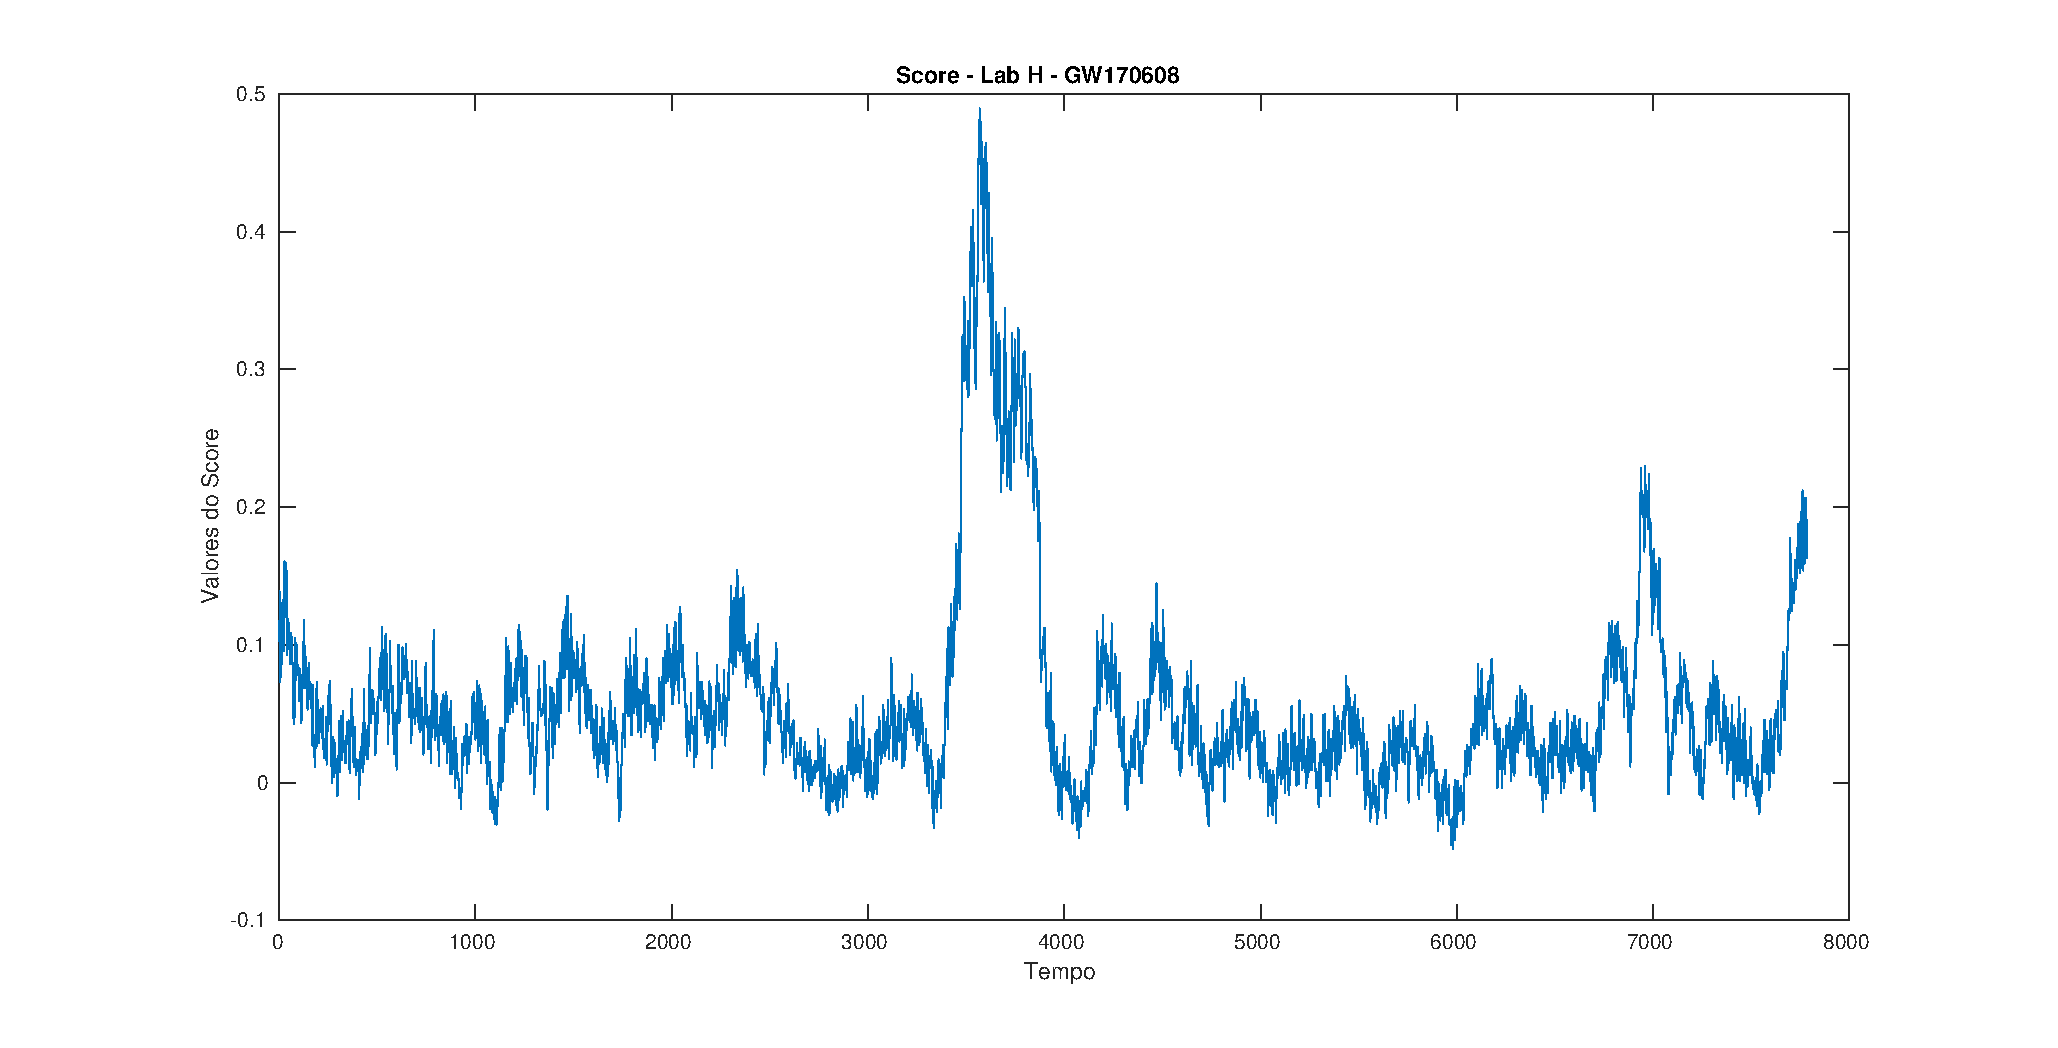
\includegraphics[width=0.5\textwidth]{figuras/GW170608_LabH.eps}}
     \subfigure[Score gerado para o laboratório L]{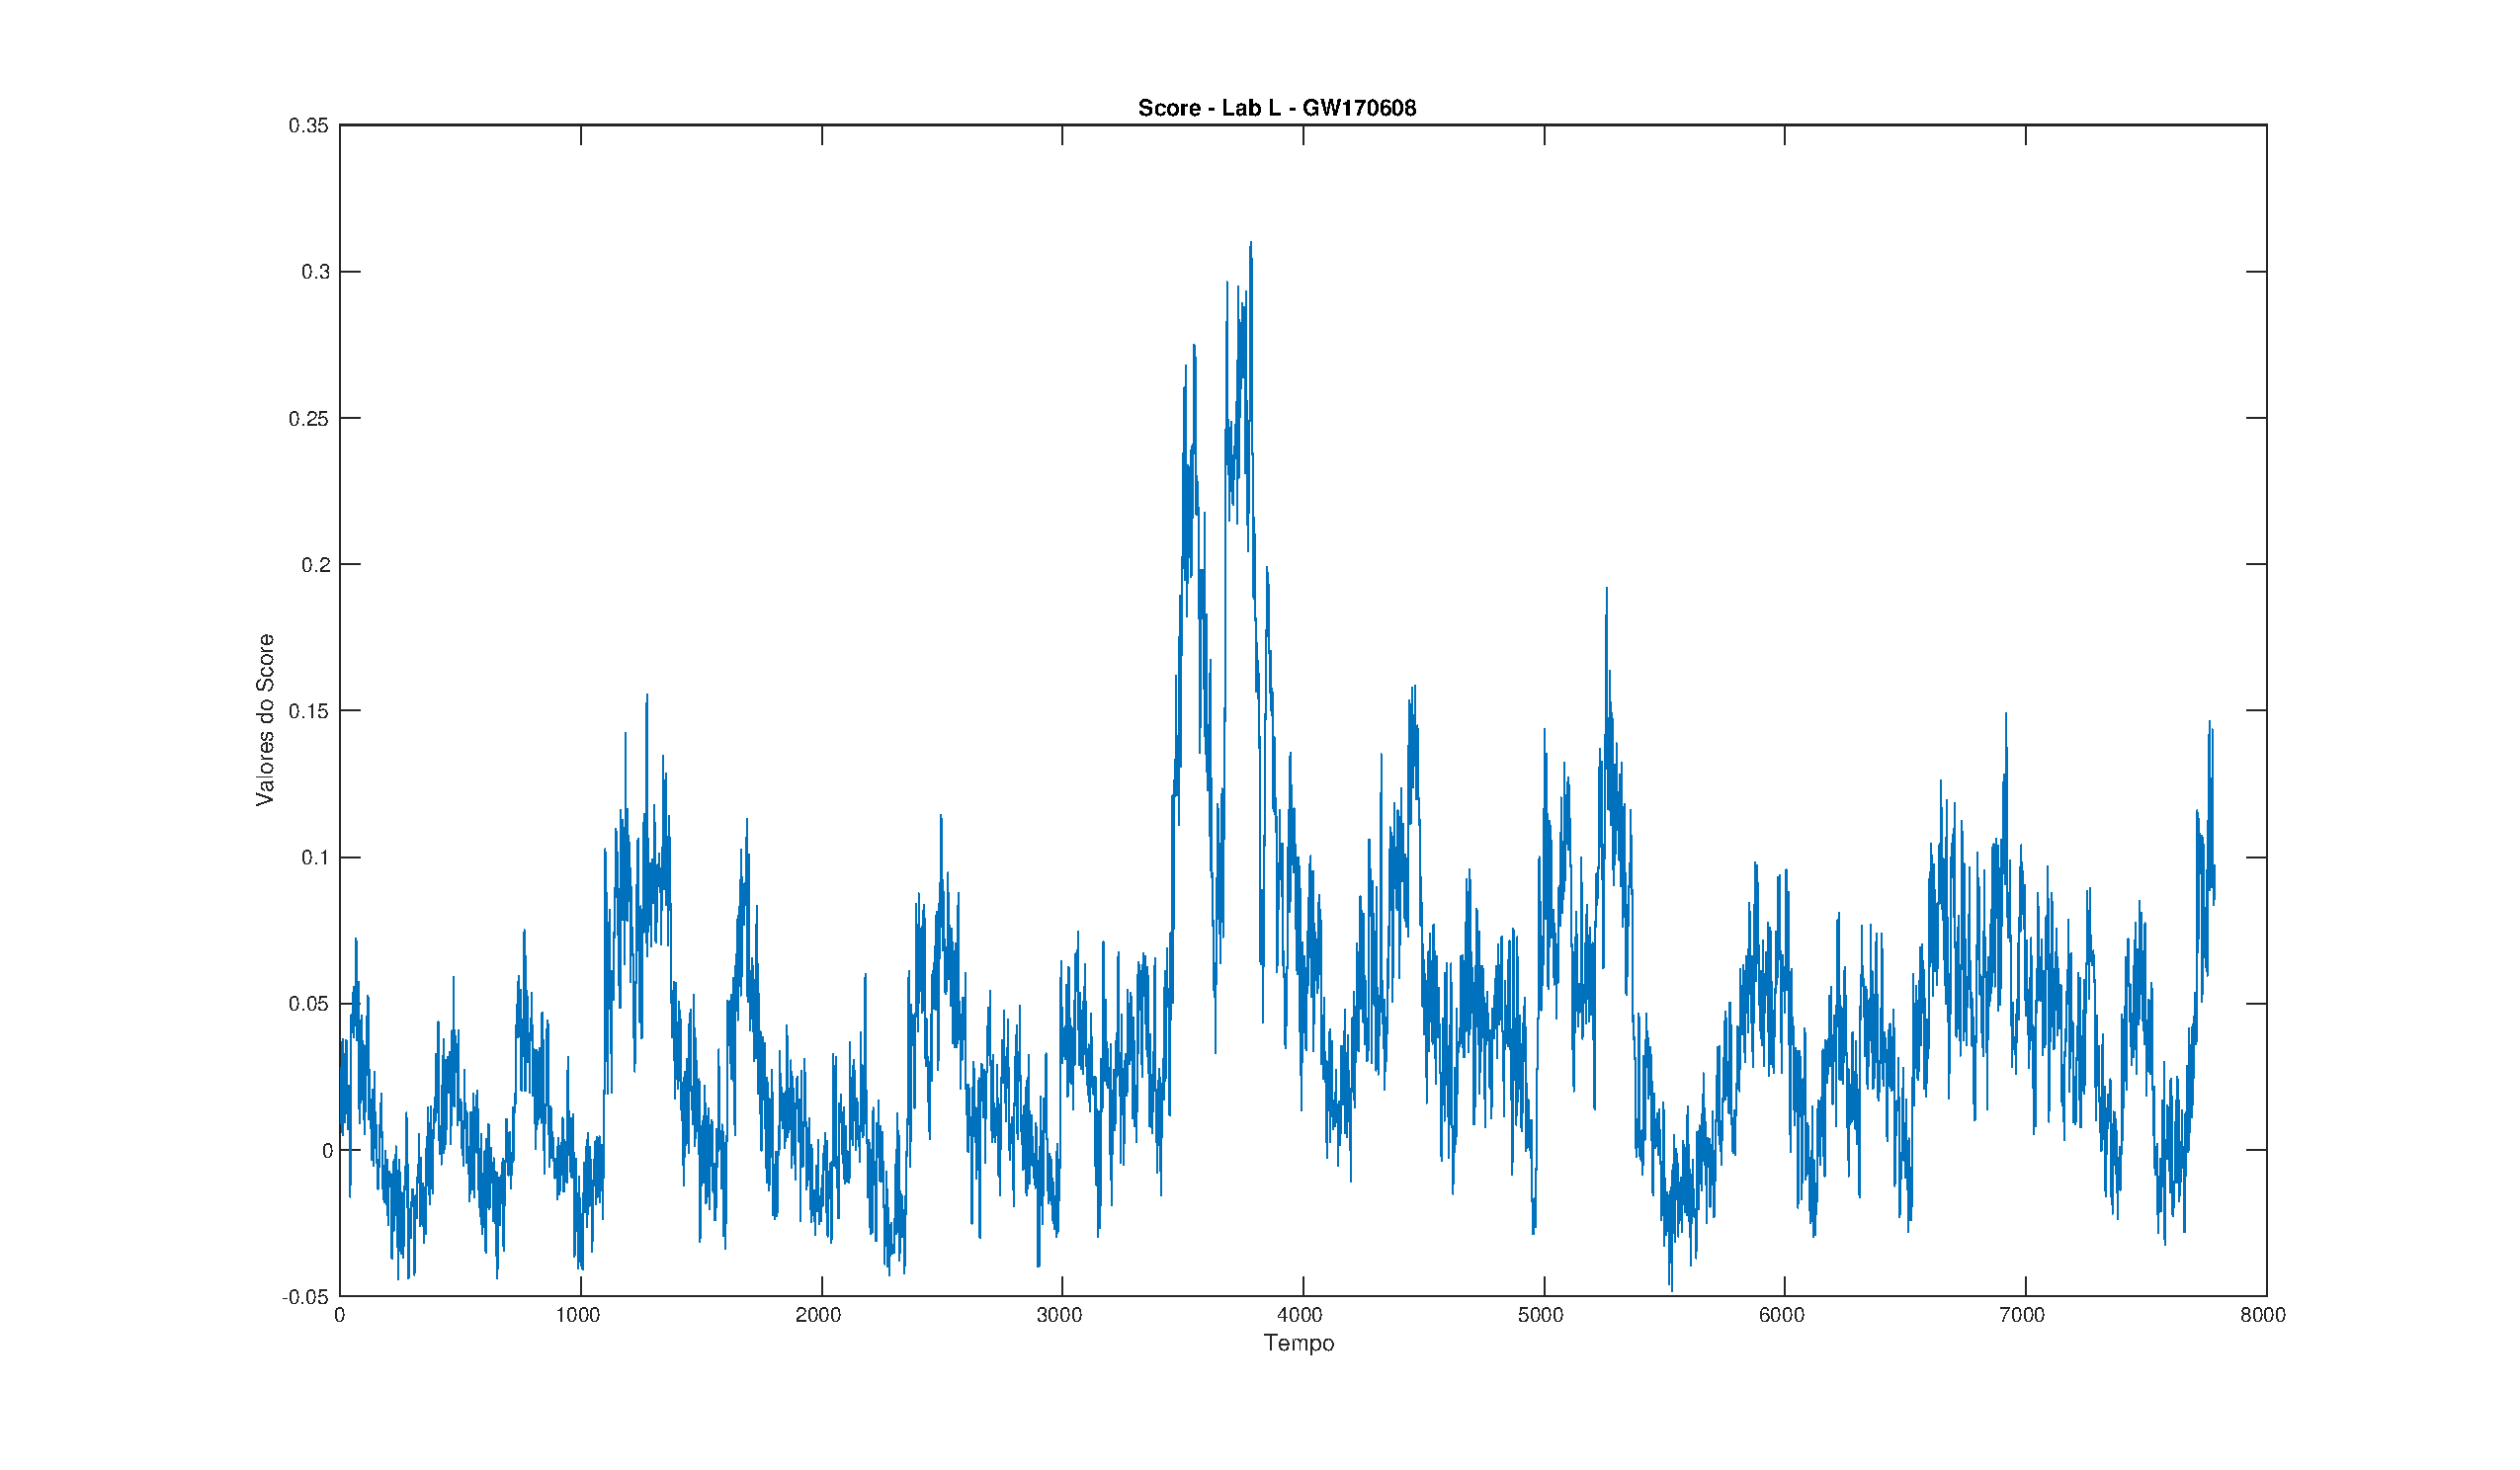
\includegraphics[width=0.5\textwidth]{figuras/GW170608_LabL.eps}}
     \subfigure[Coincidência entre os dois scores]{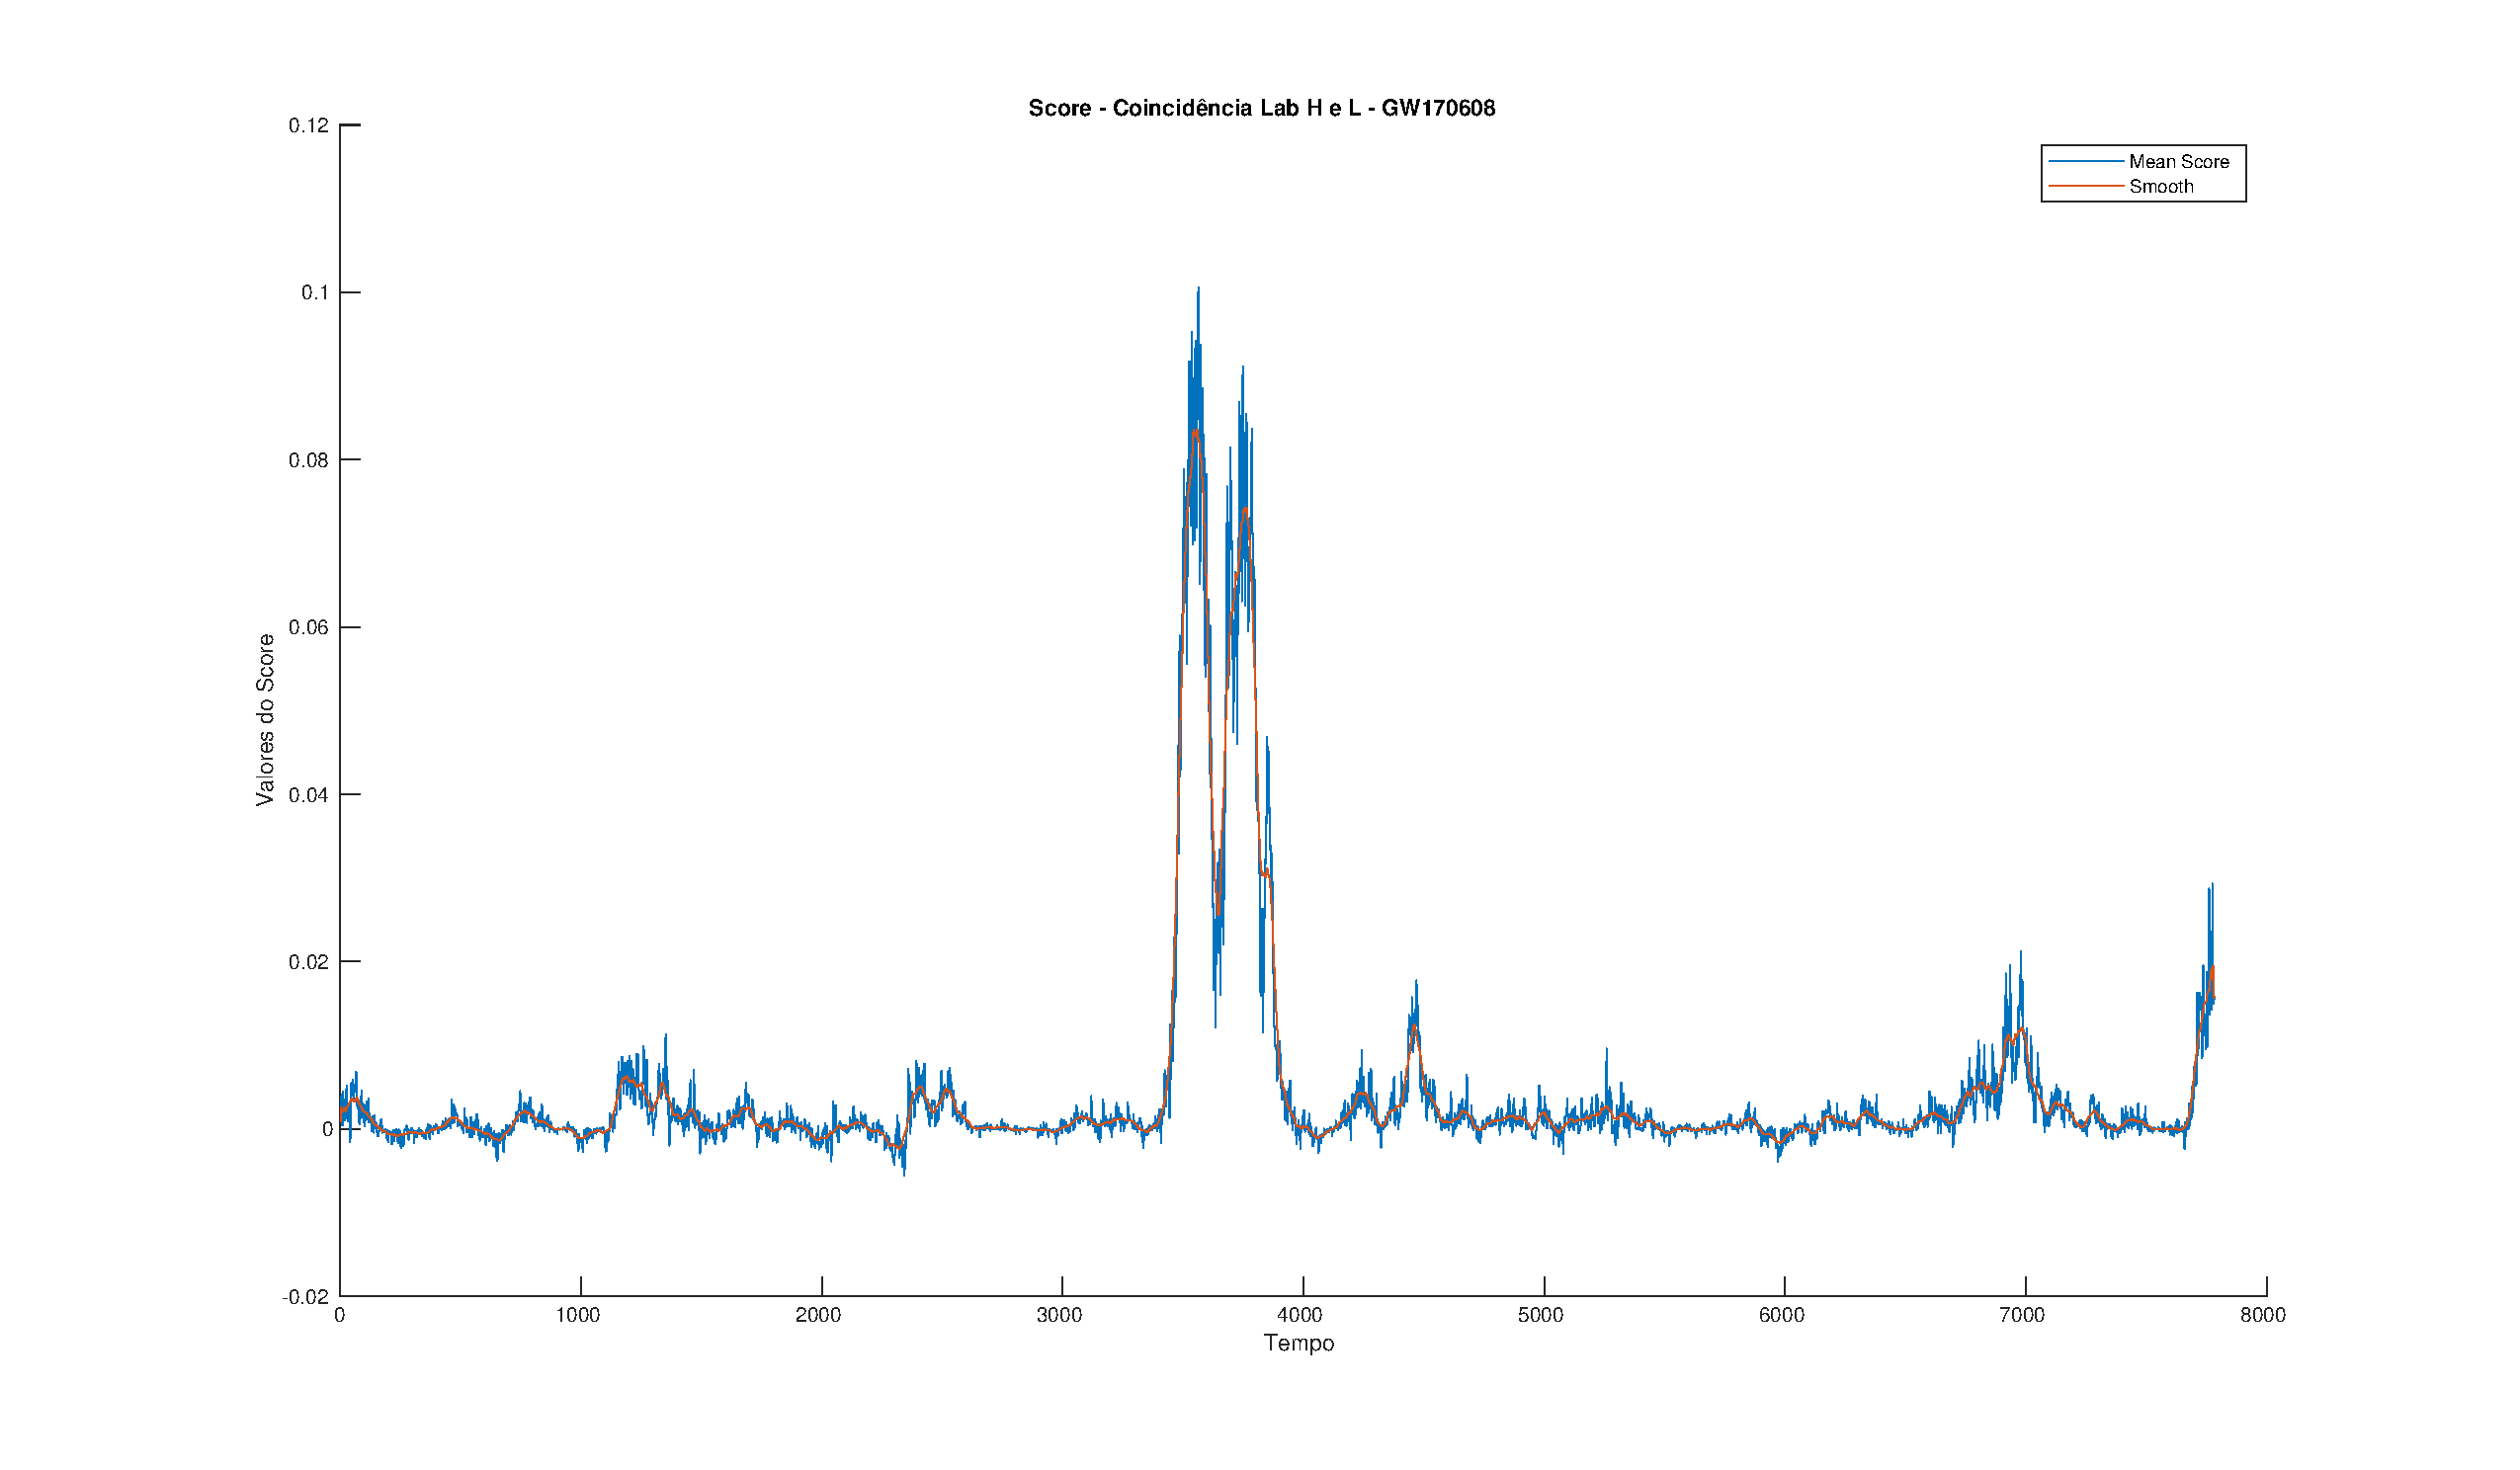
\includegraphics[width=1.0\textwidth]{figuras/GW170608_LabHL.eps}}
     \caption{Score da onda gravitacional GW170608}
 \end{figure}
 
\section{Score da onda gravitacional GW170729}
\begin{figure}[H]
     \subfigure[Score gerado para o laboratório H]{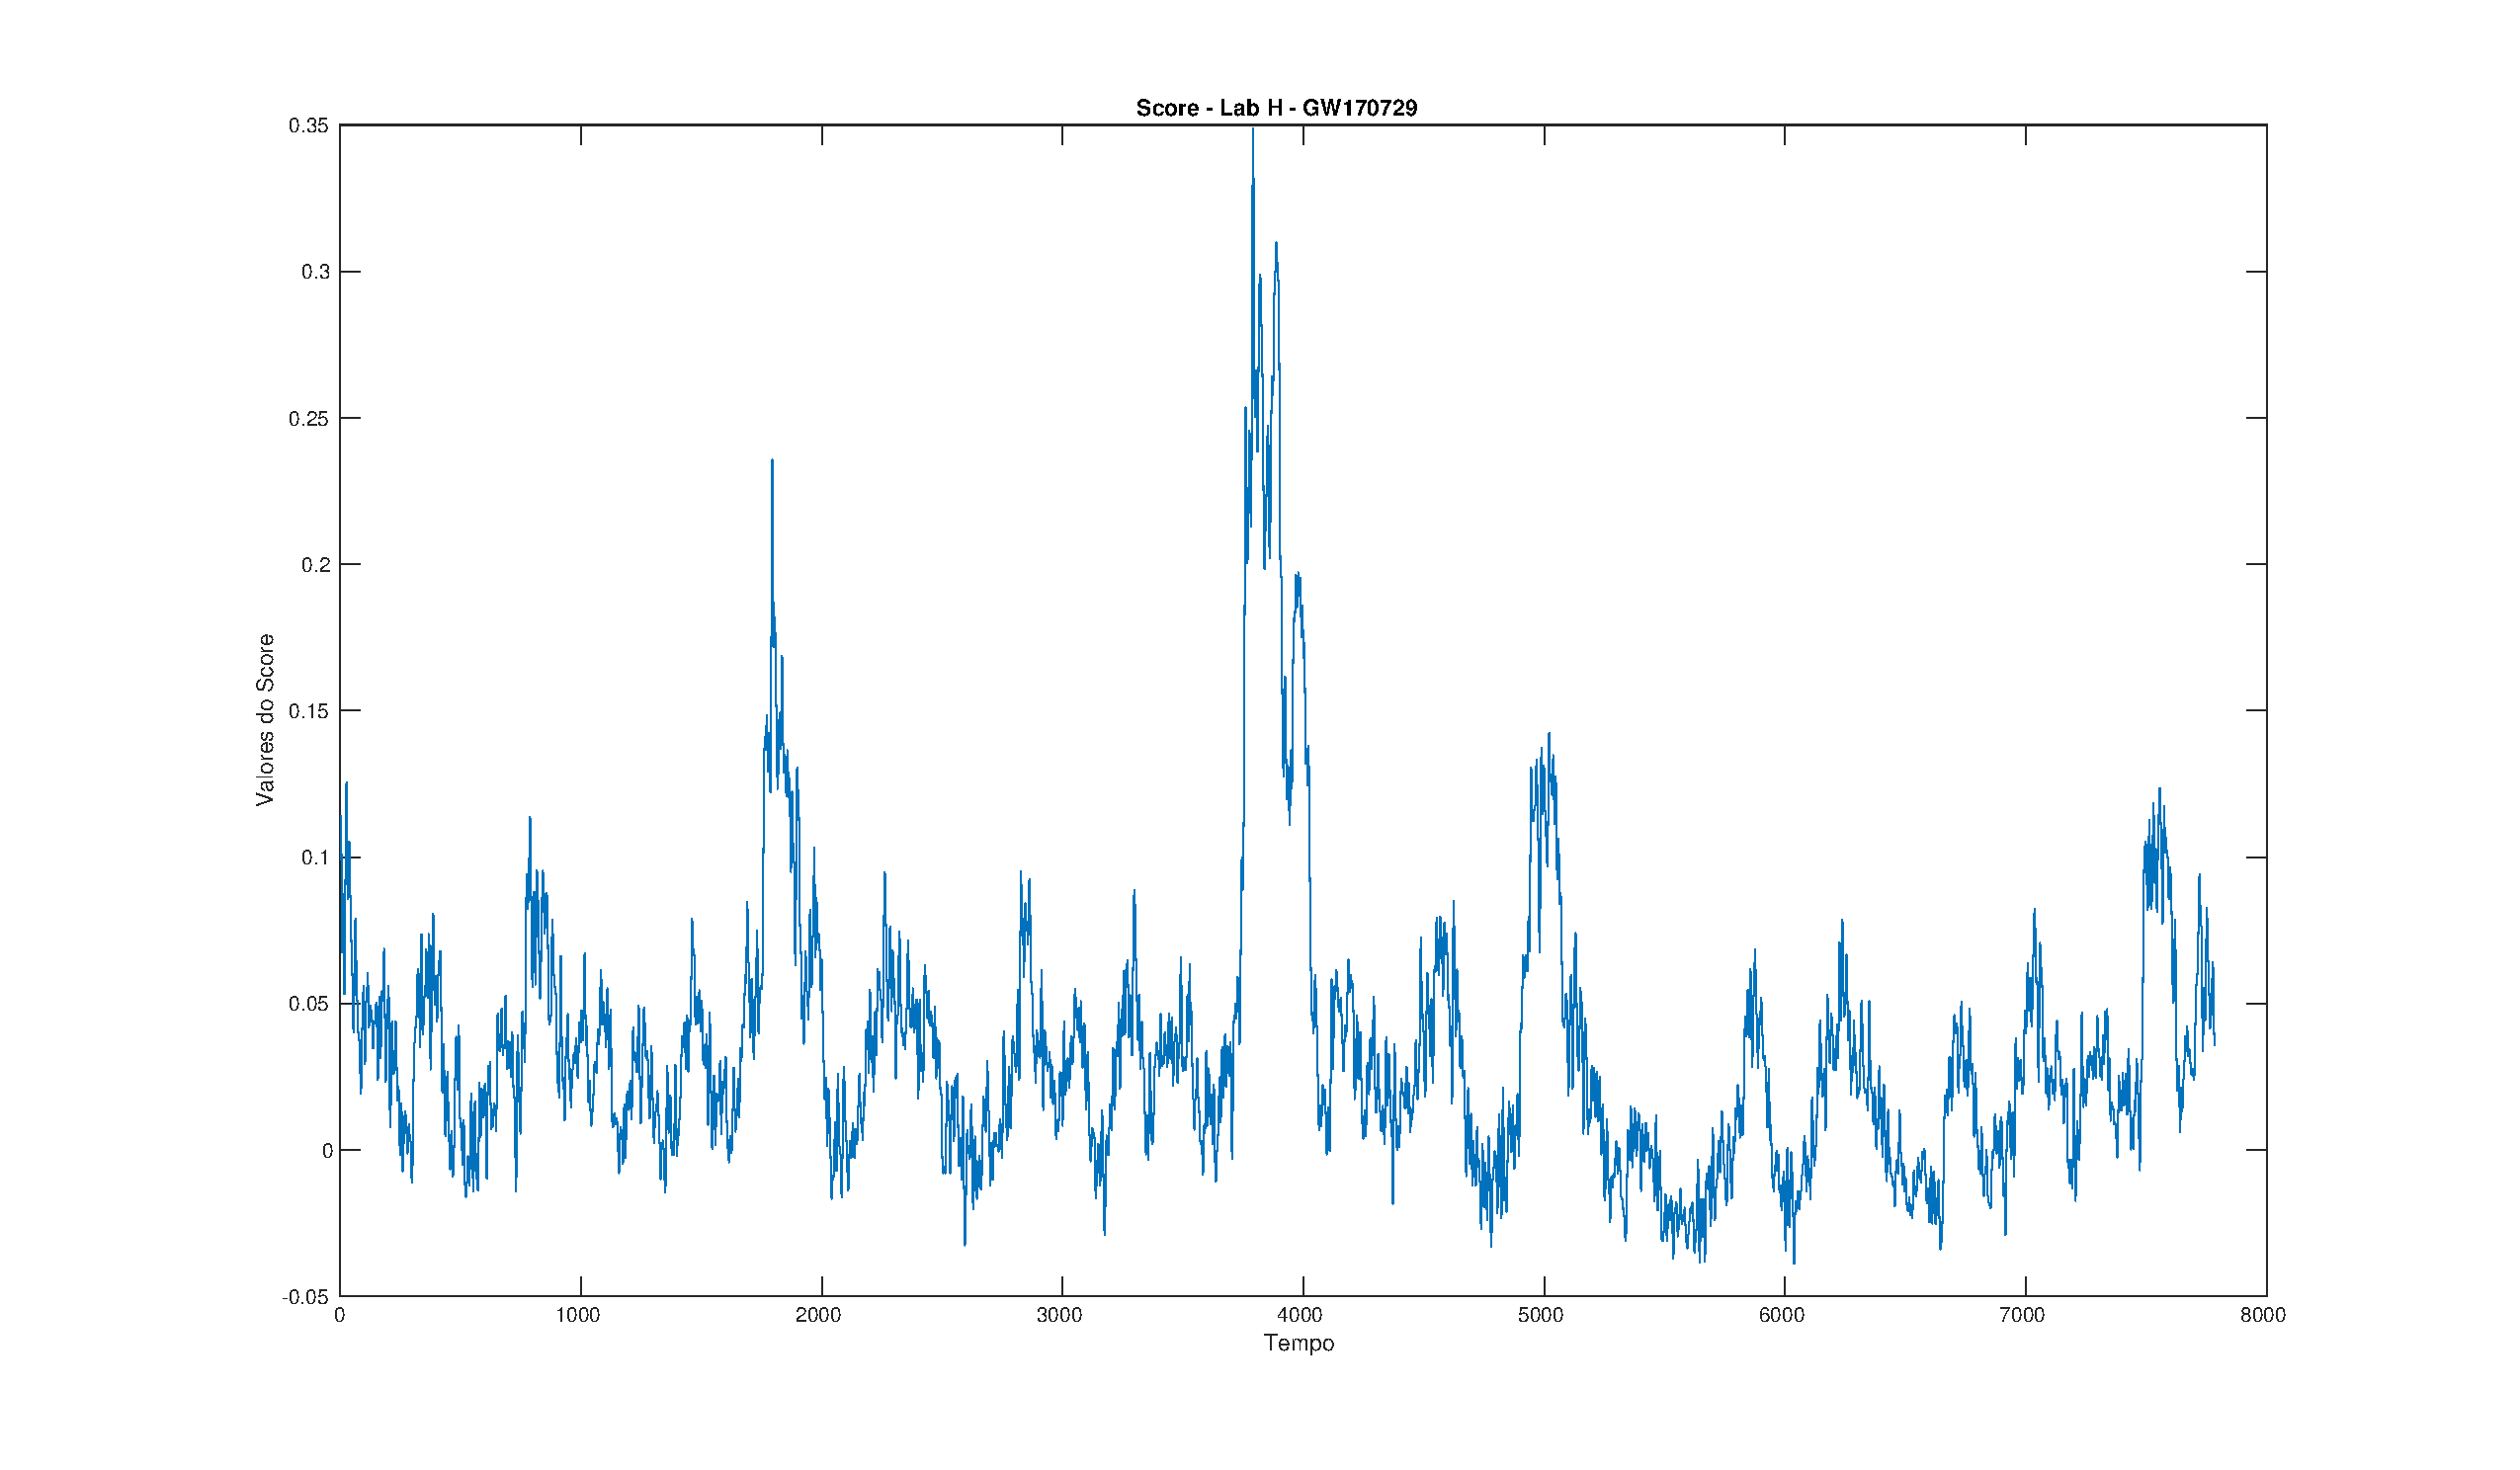
\includegraphics[width=0.5\textwidth]{figuras/GW170729_LabH.eps}}
     \subfigure[Score gerado para o laboratório L]{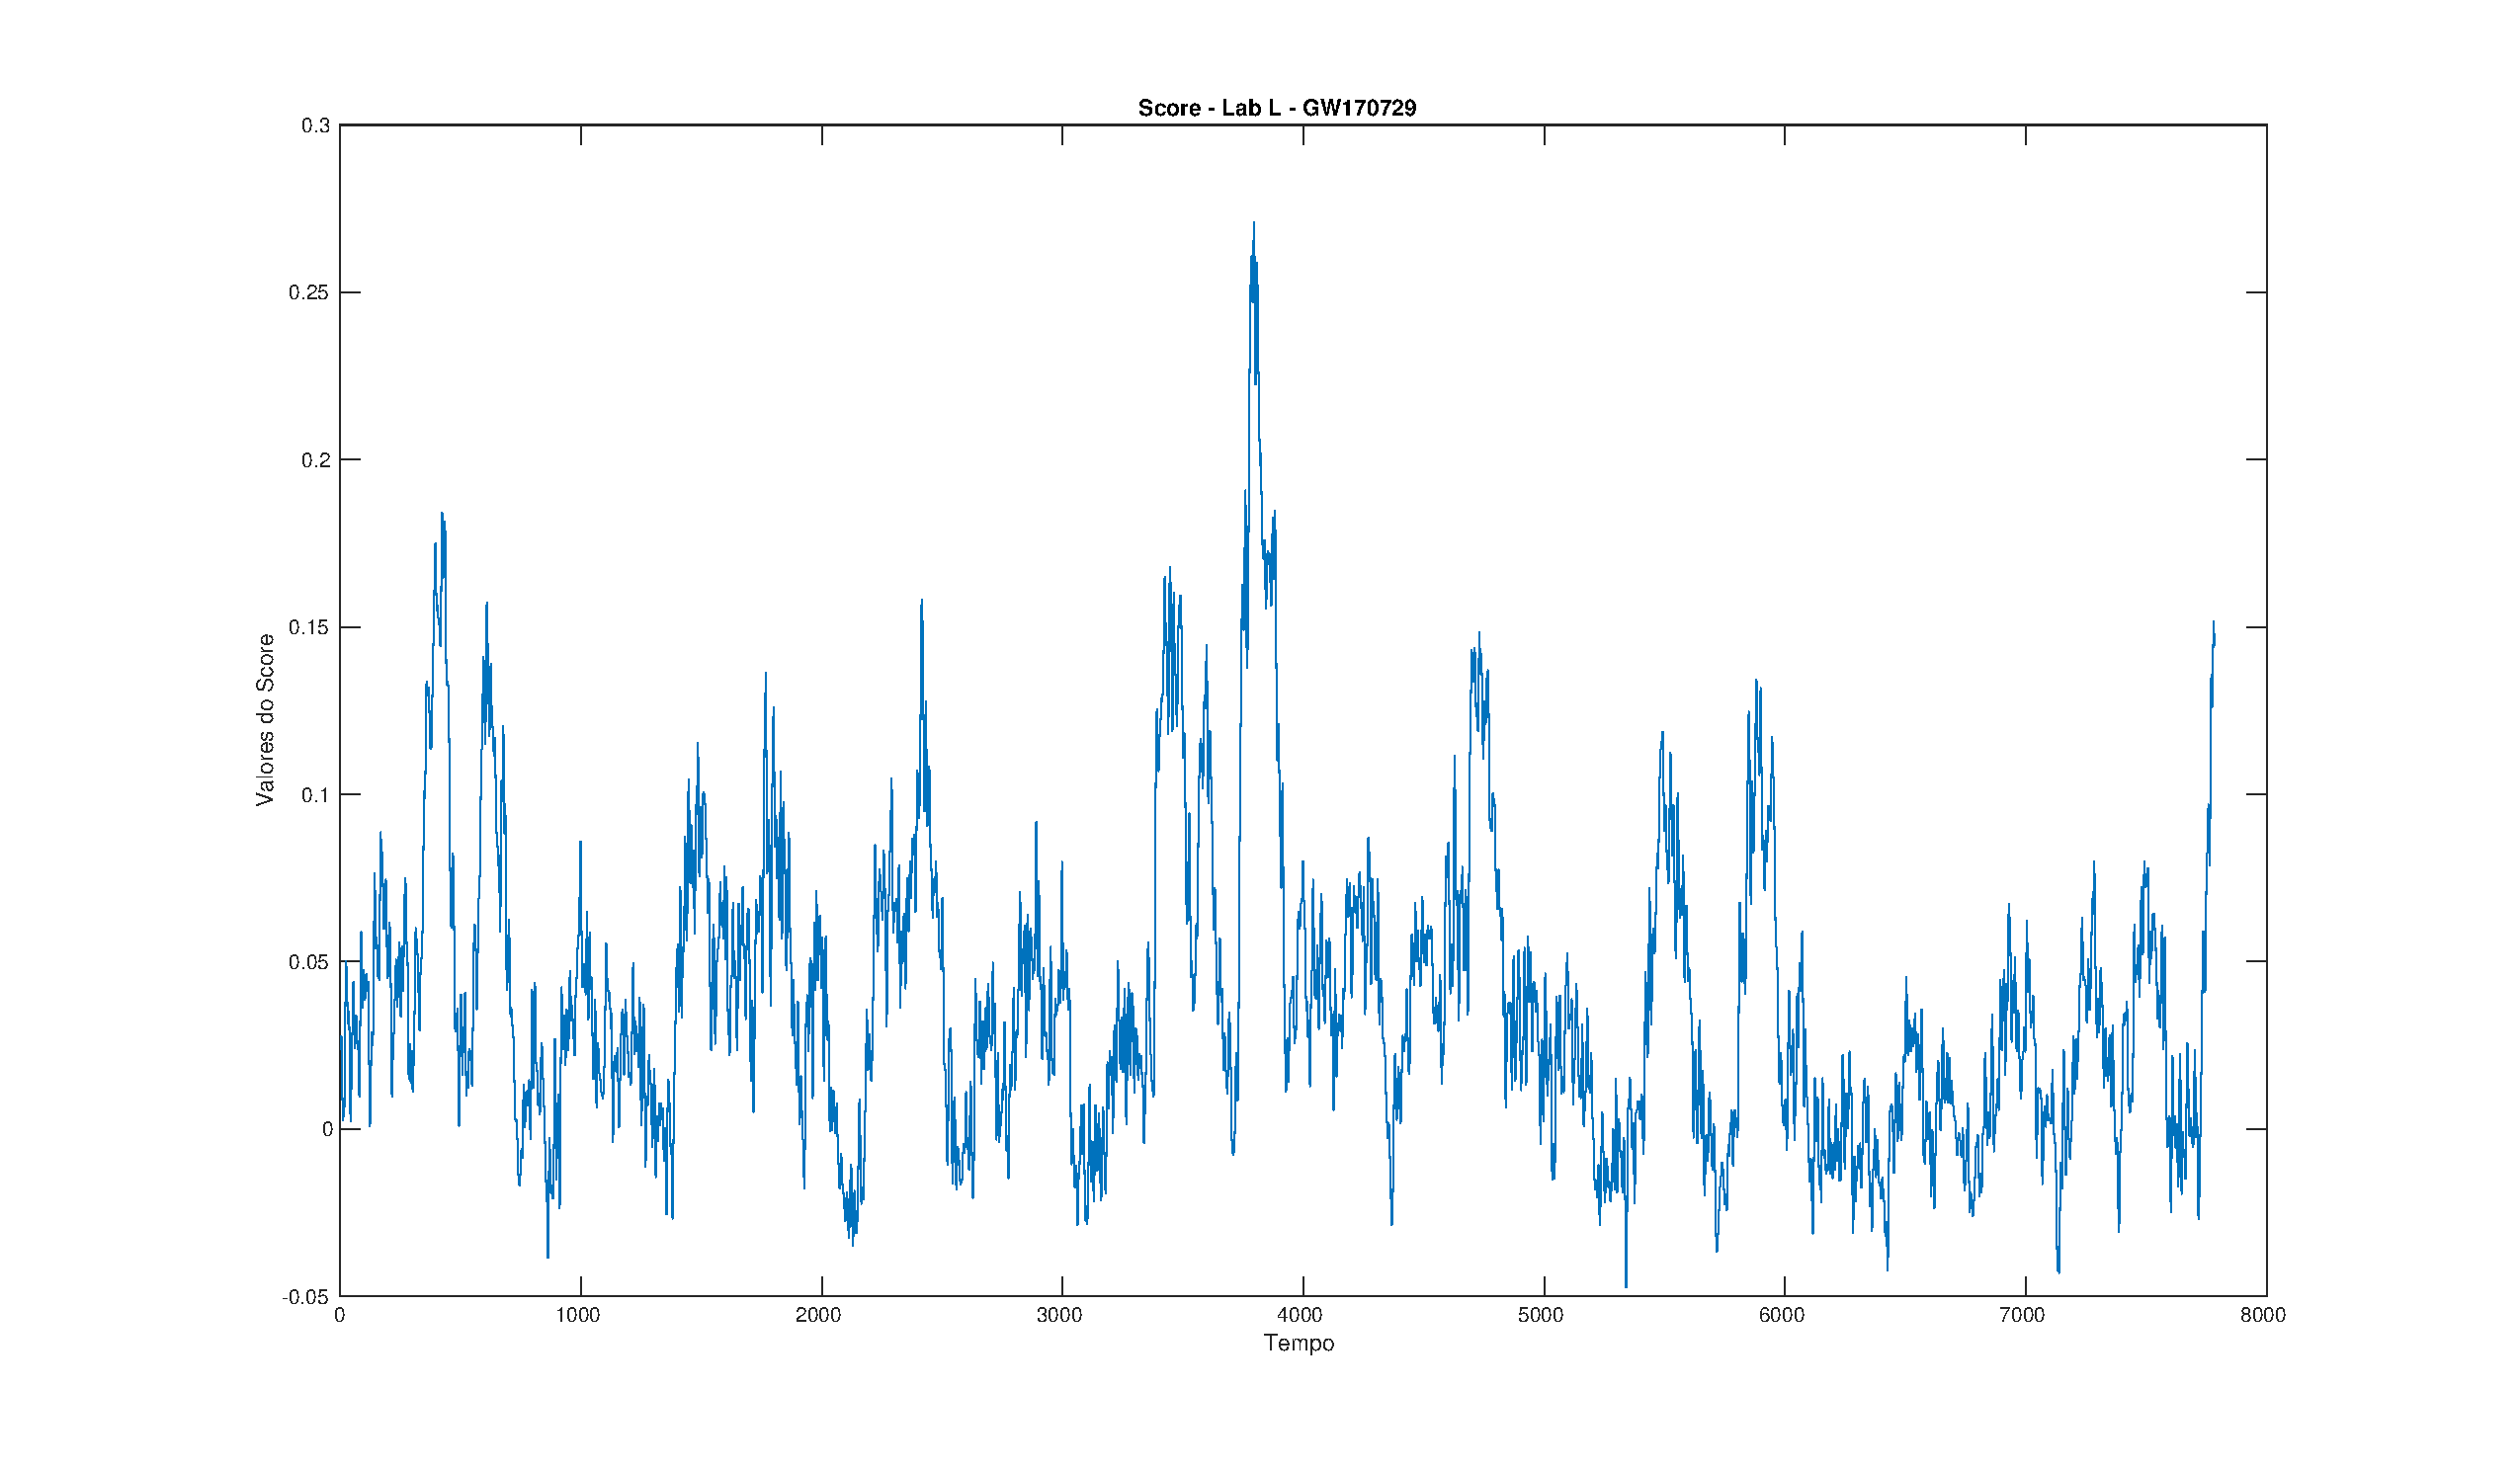
\includegraphics[width=0.5\textwidth]{figuras/GW170729_LabL.eps}}
     \subfigure[Coincidência entre os dois scores]{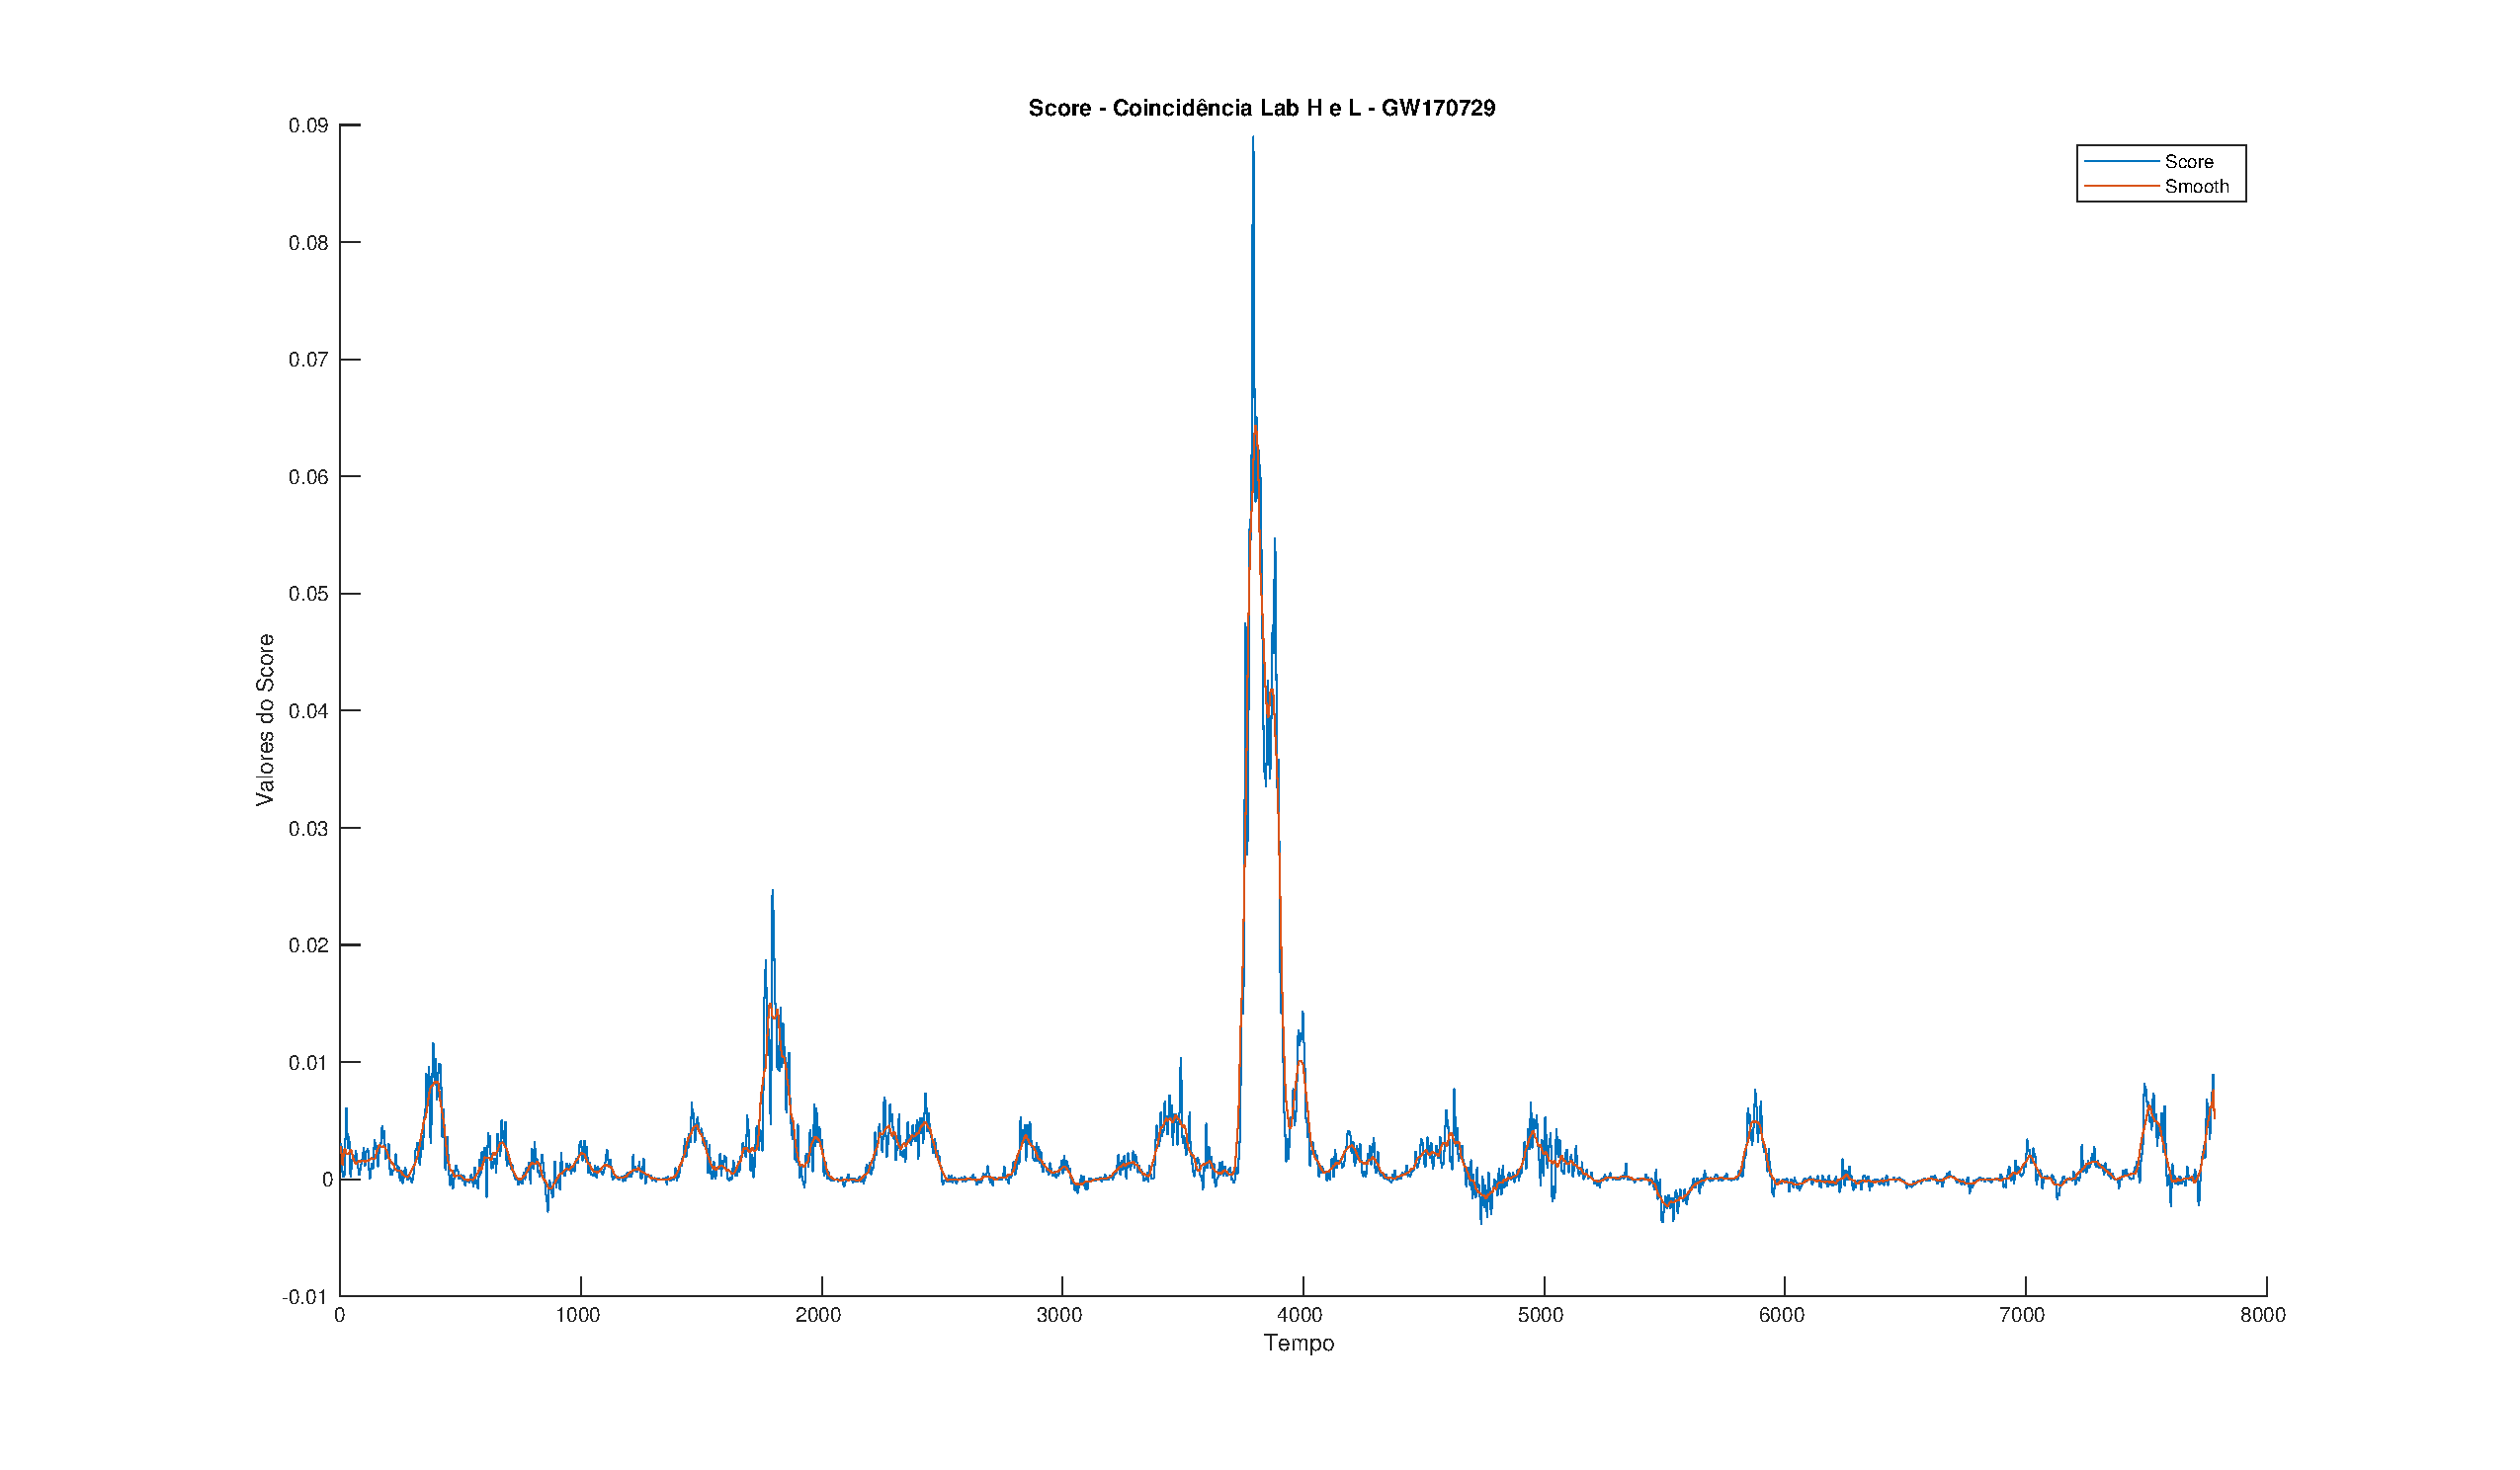
\includegraphics[width=1.0\textwidth]{figuras/GW170729_LabHL.eps}}
     \caption{Score da onda gravitacional GW170729}
 \end{figure}
 
\section{Score da onda gravitacional GW170809}
\begin{figure}[H]
     \subfigure[Score gerado para o laboratório H]{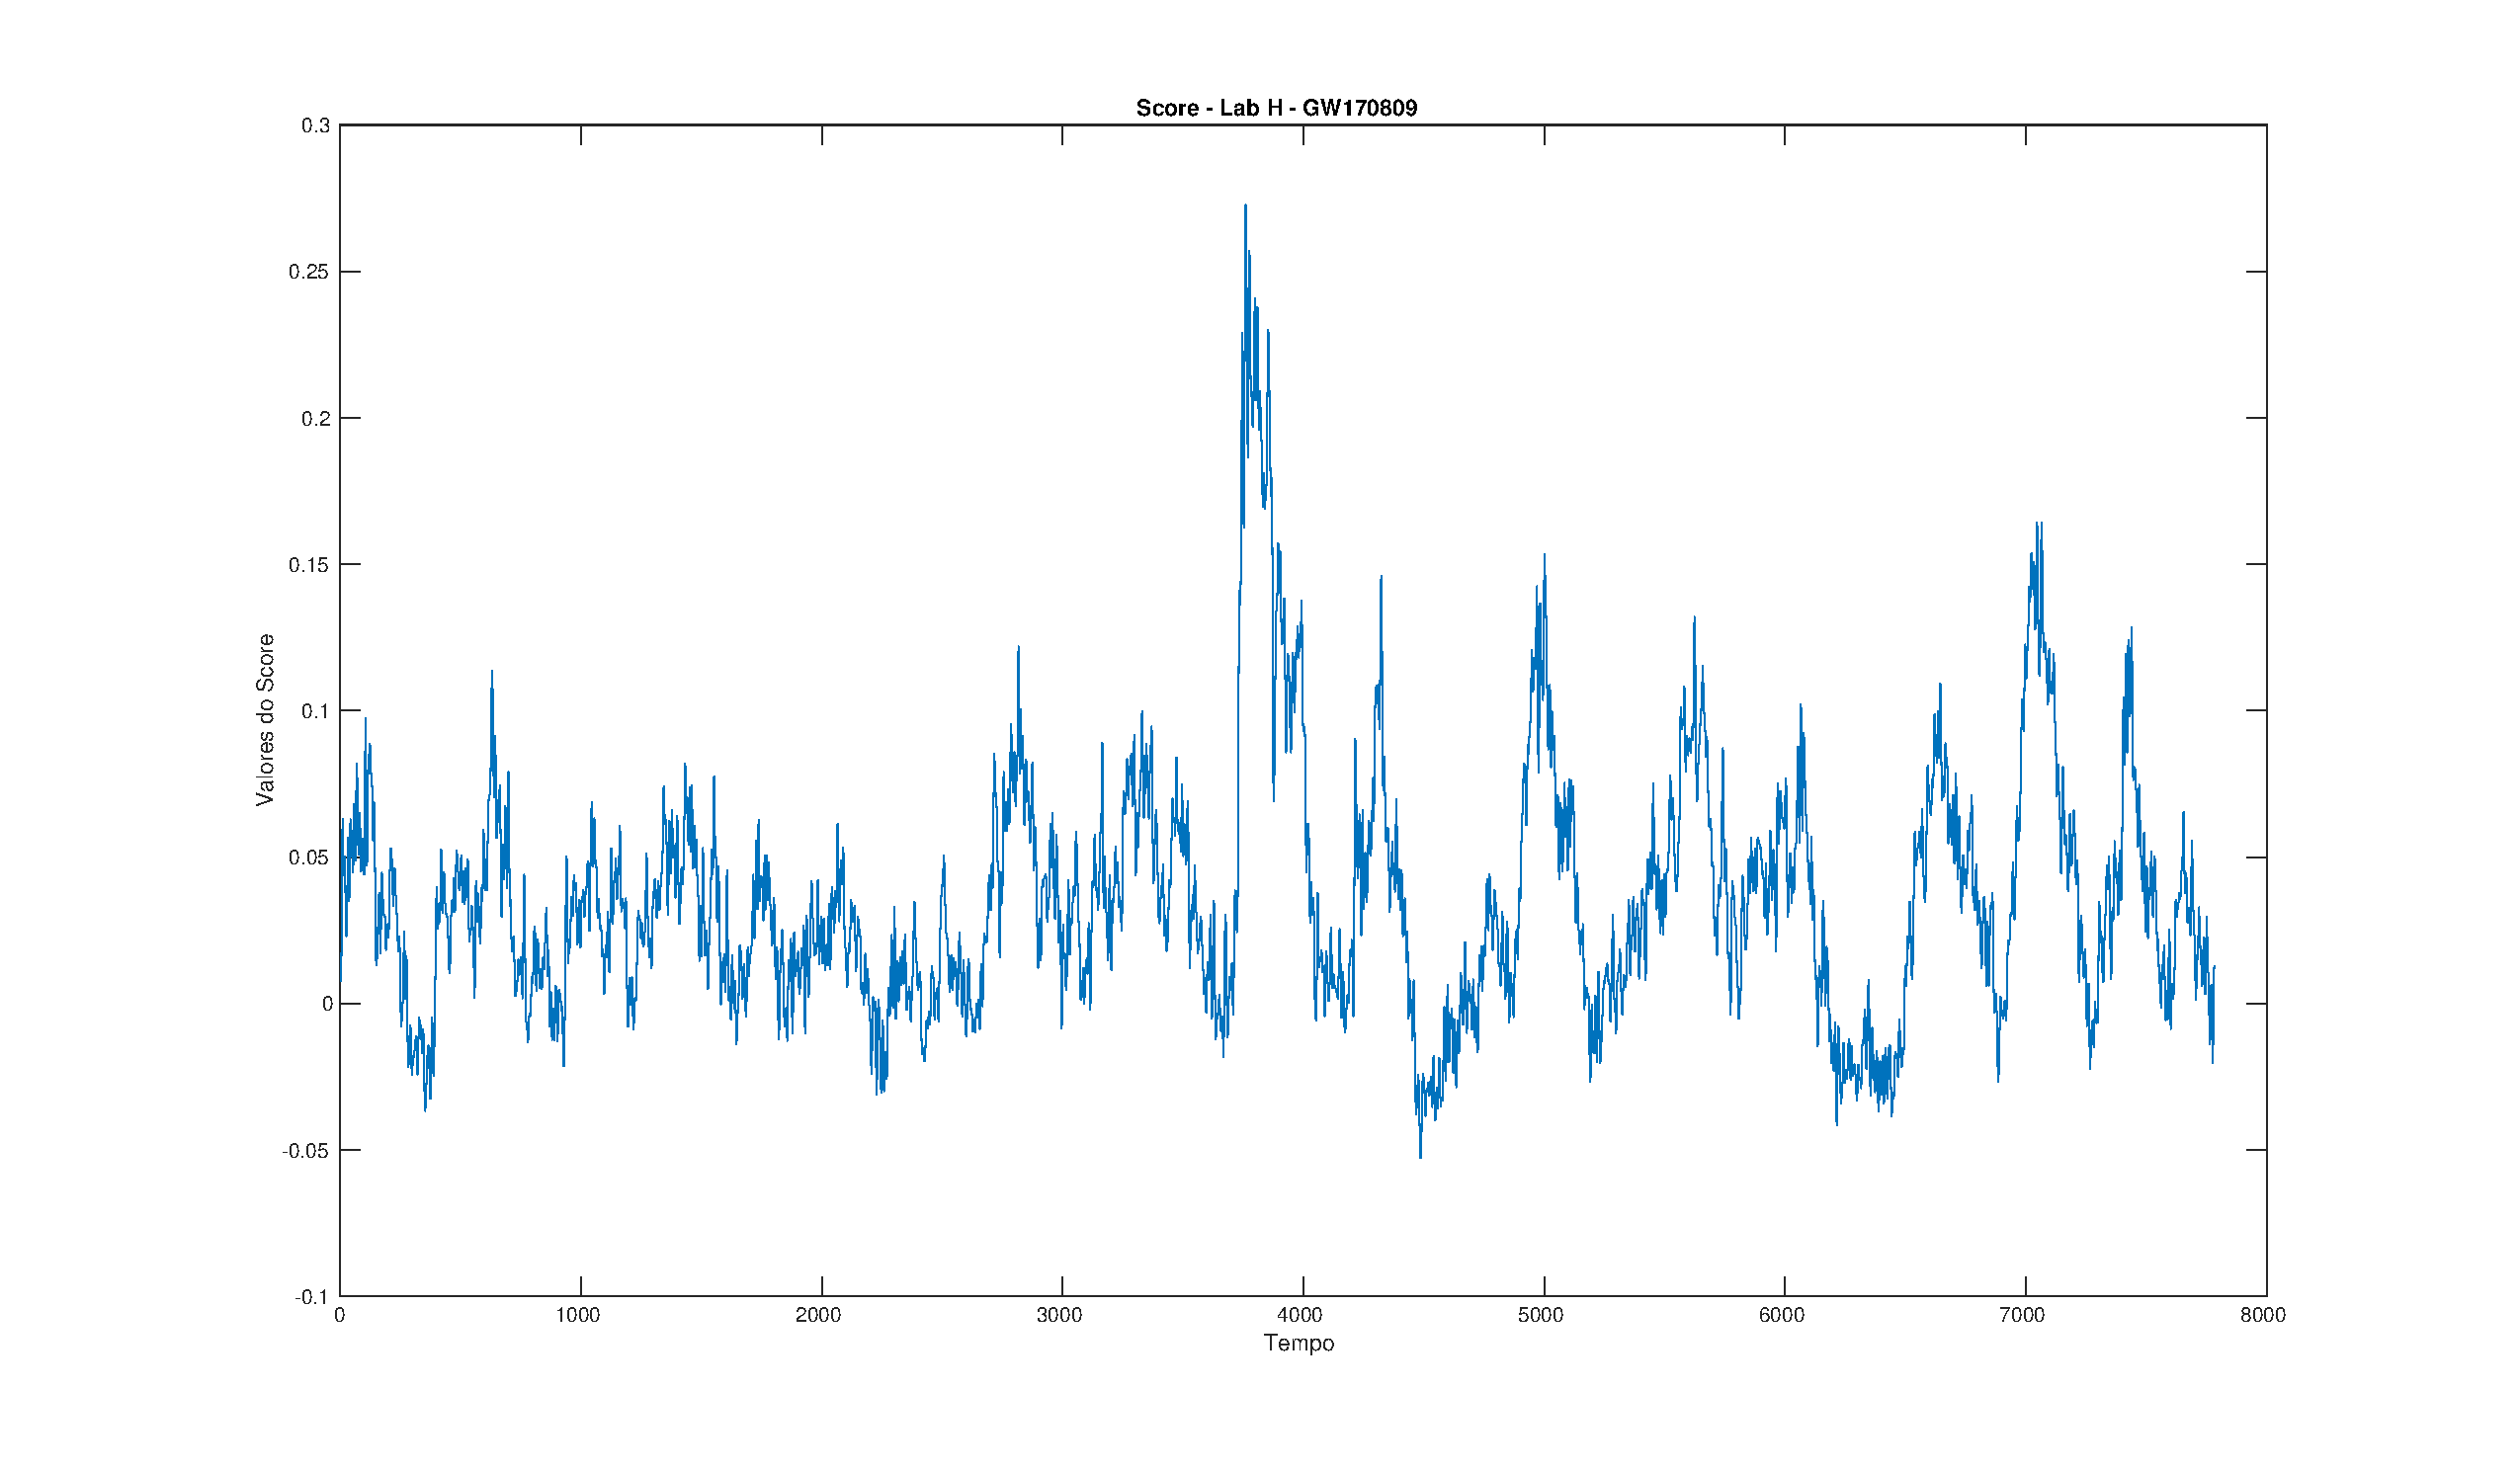
\includegraphics[width=0.5\textwidth]{figuras/GW170809_LabH.eps}}
     \subfigure[Score gerado para o laboratório L]{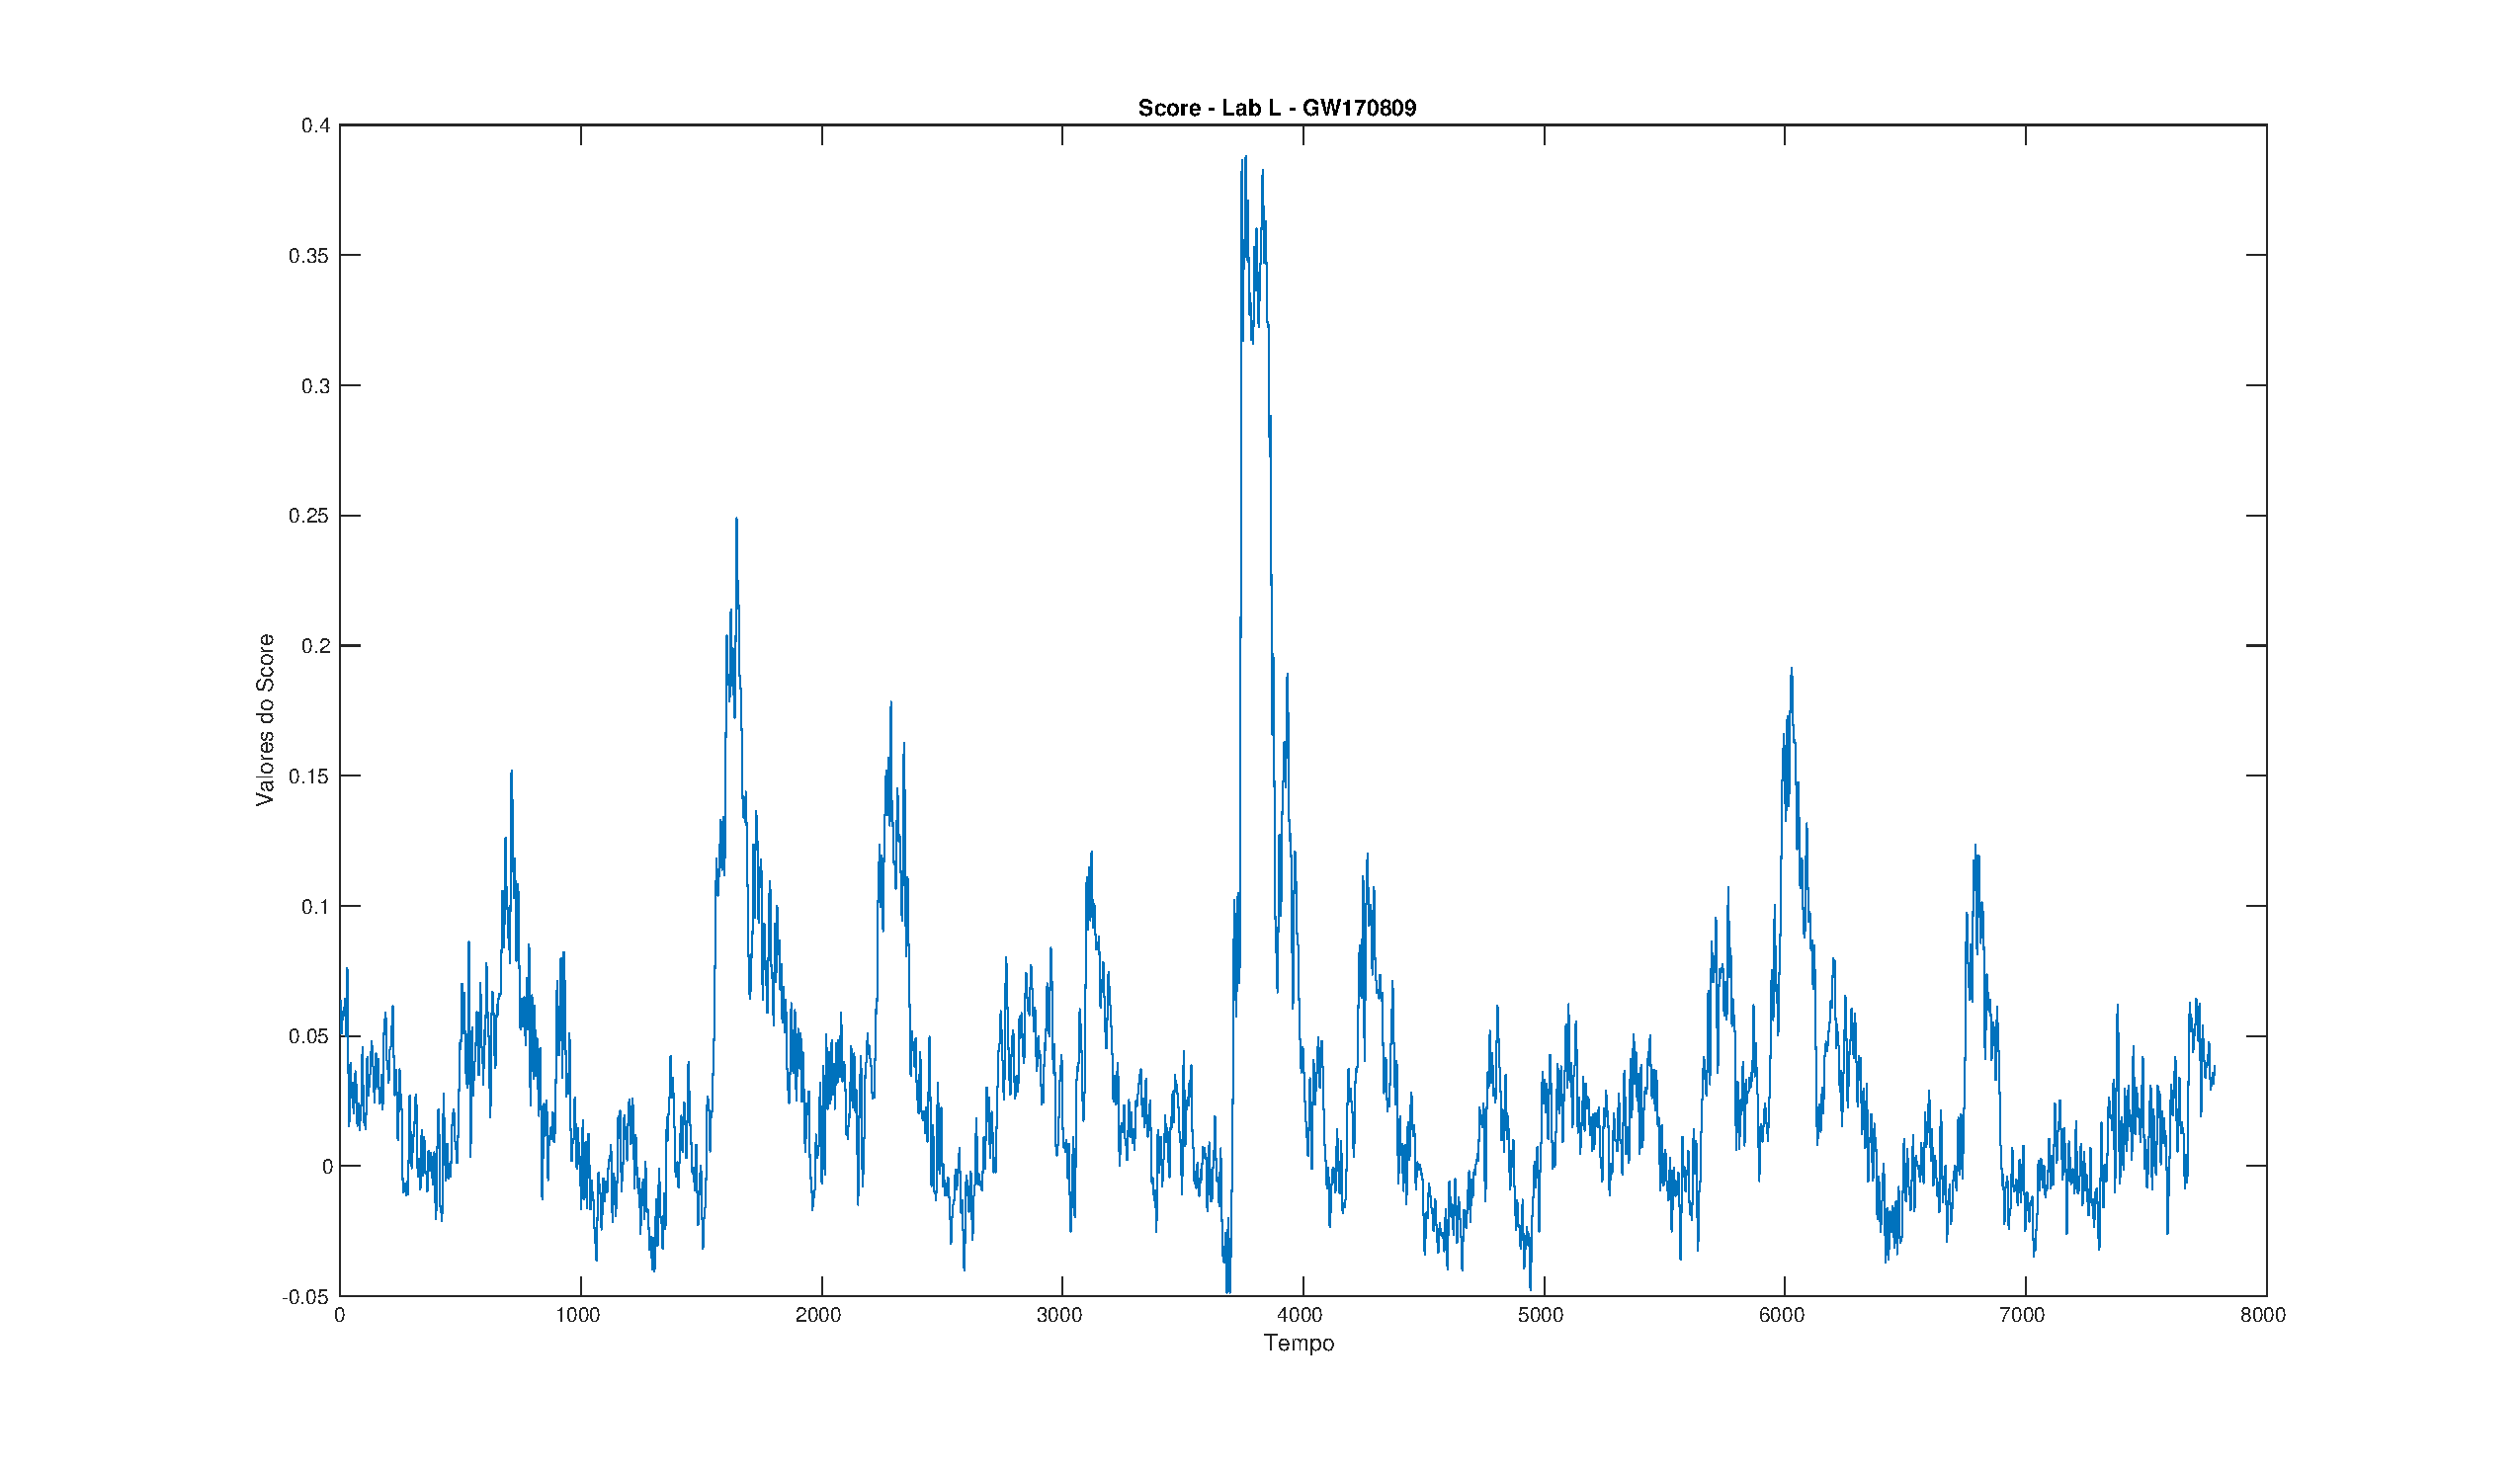
\includegraphics[width=0.5\textwidth]{figuras/GW170809_LabL.eps}}
     \subfigure[Coincidência entre os dois scores]{\includegraphics[width=1.0\textwidth]{figuras/GW170809_LabHL.eps}}
     \caption{Score da onda gravitacional GW170809}
 \end{figure}
 
\section{Score da onda gravitacional GW170814}
\begin{figure}[H]
     \subfigure[Score gerado para o laboratório H]{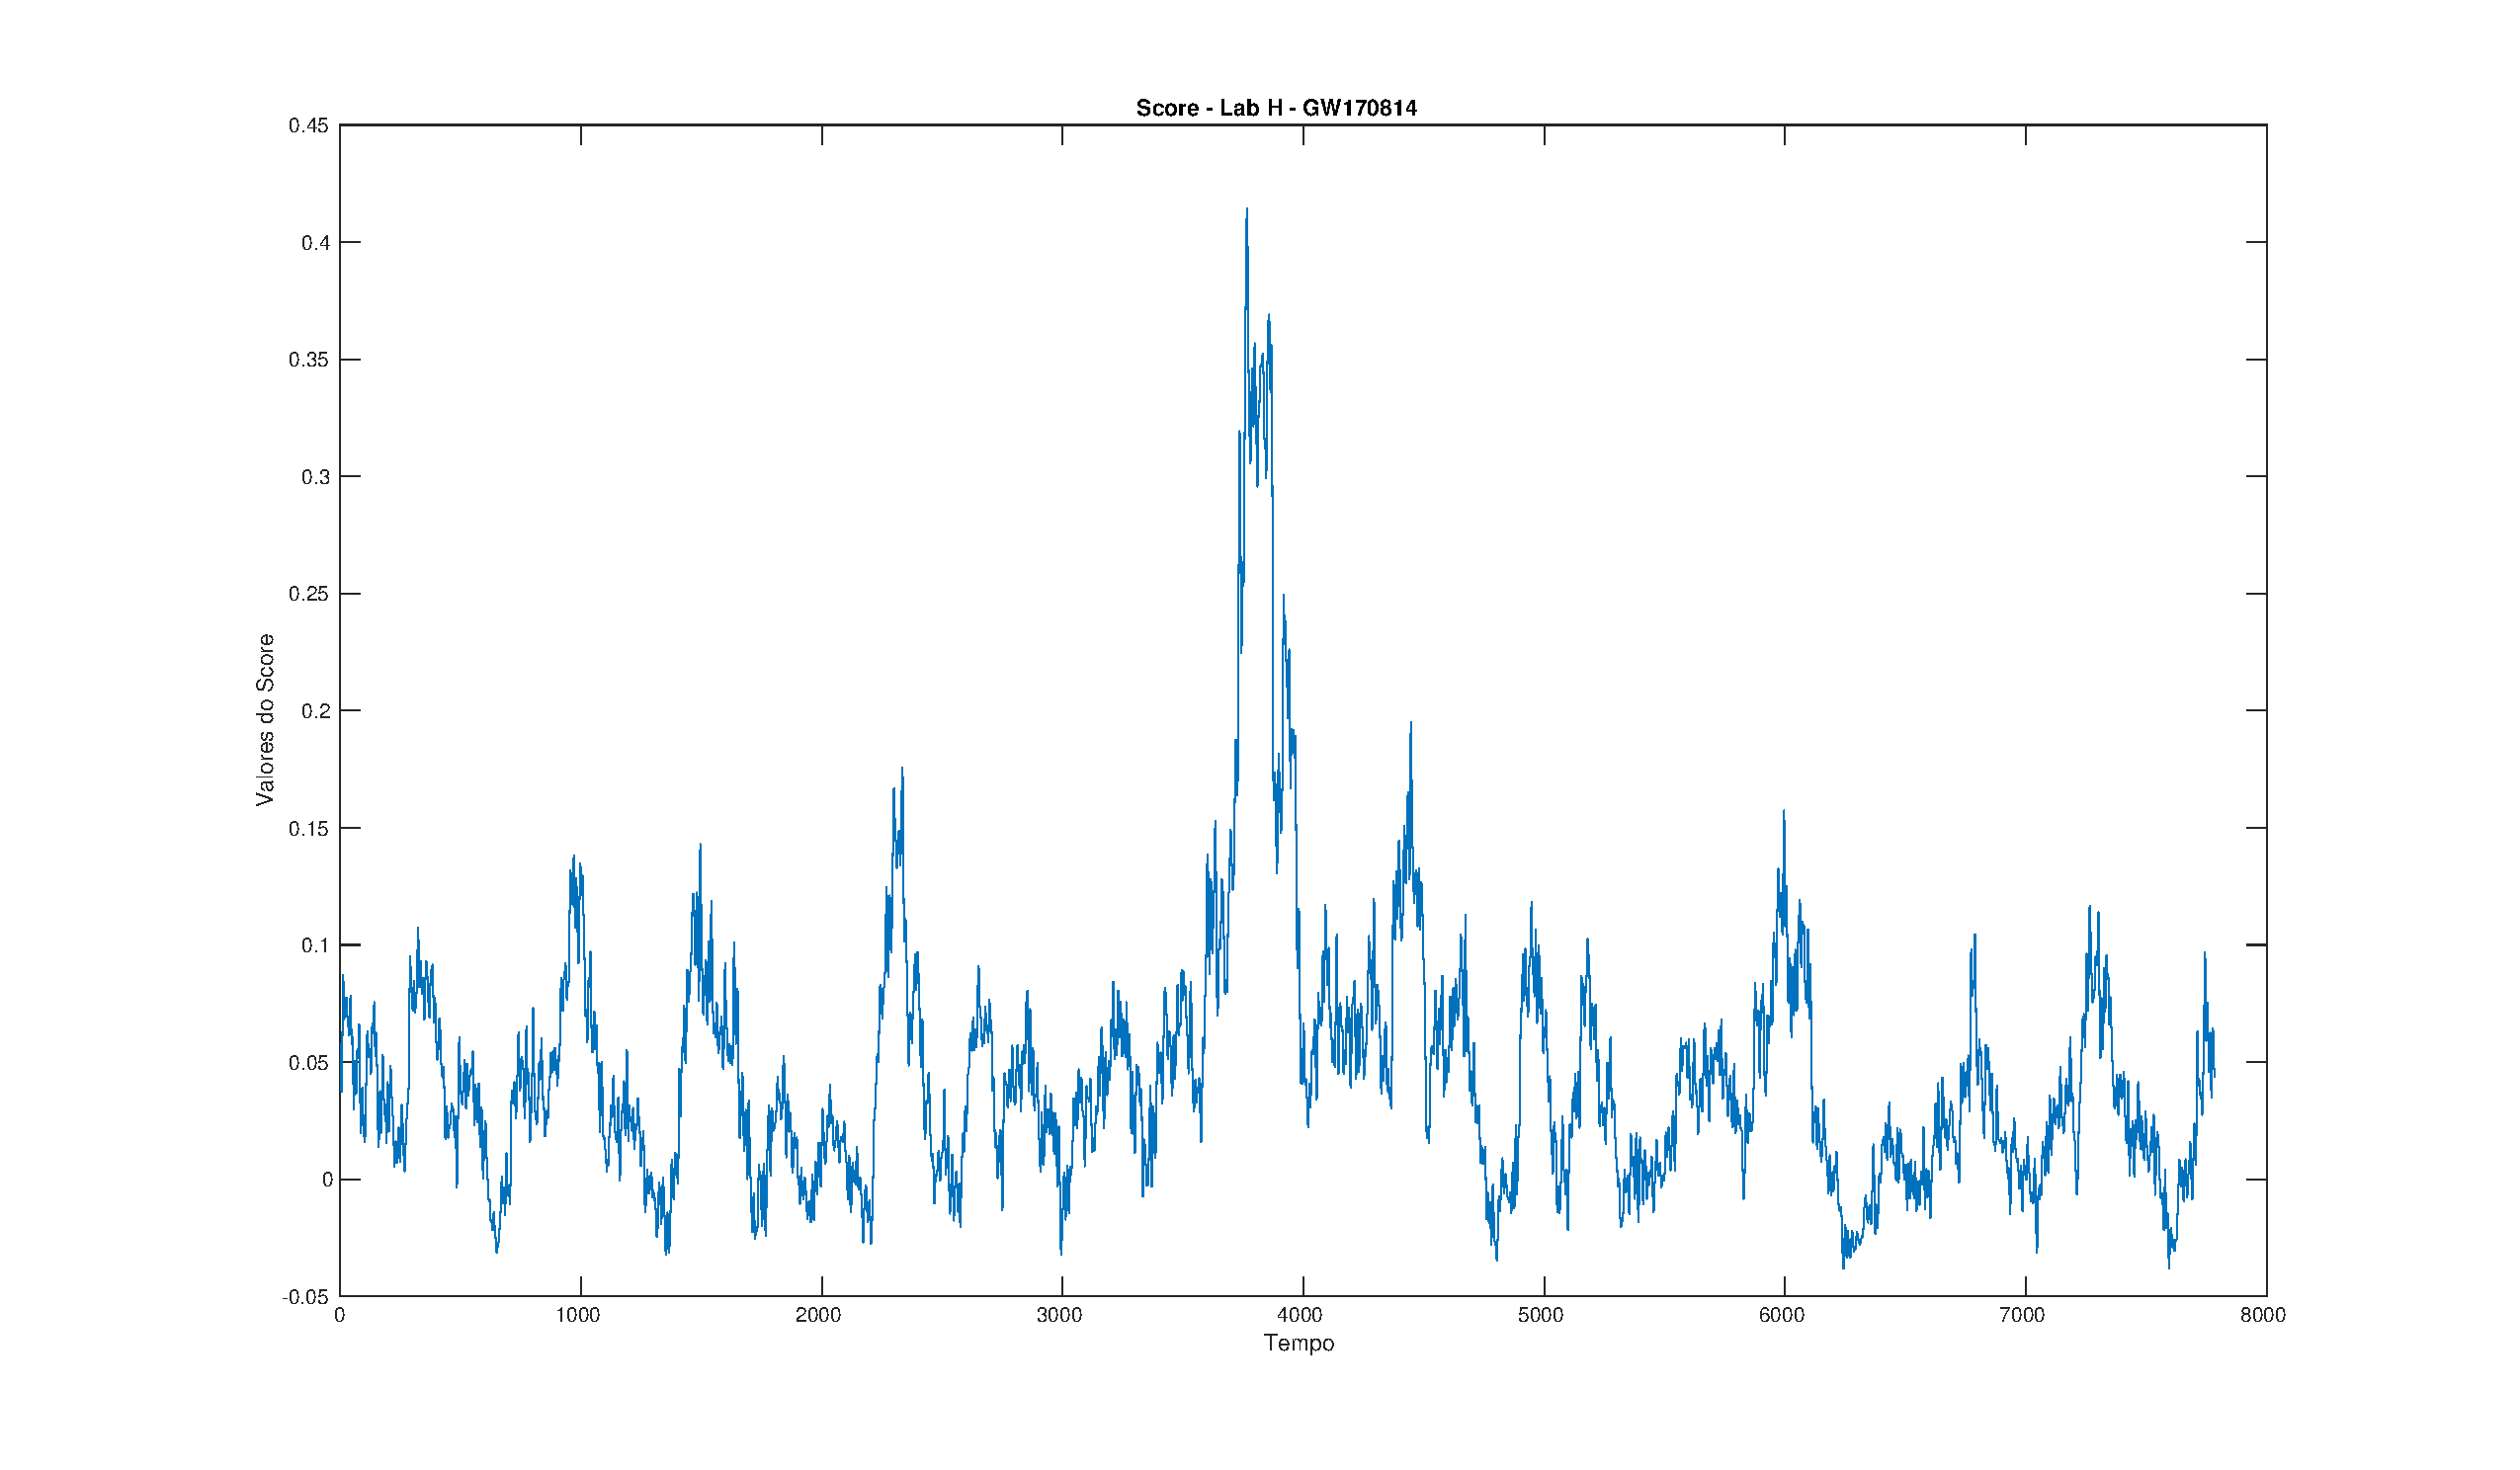
\includegraphics[width=0.5\textwidth]{figuras/GW170814_LabH.eps}}
     \subfigure[Score gerado para o laboratório L]{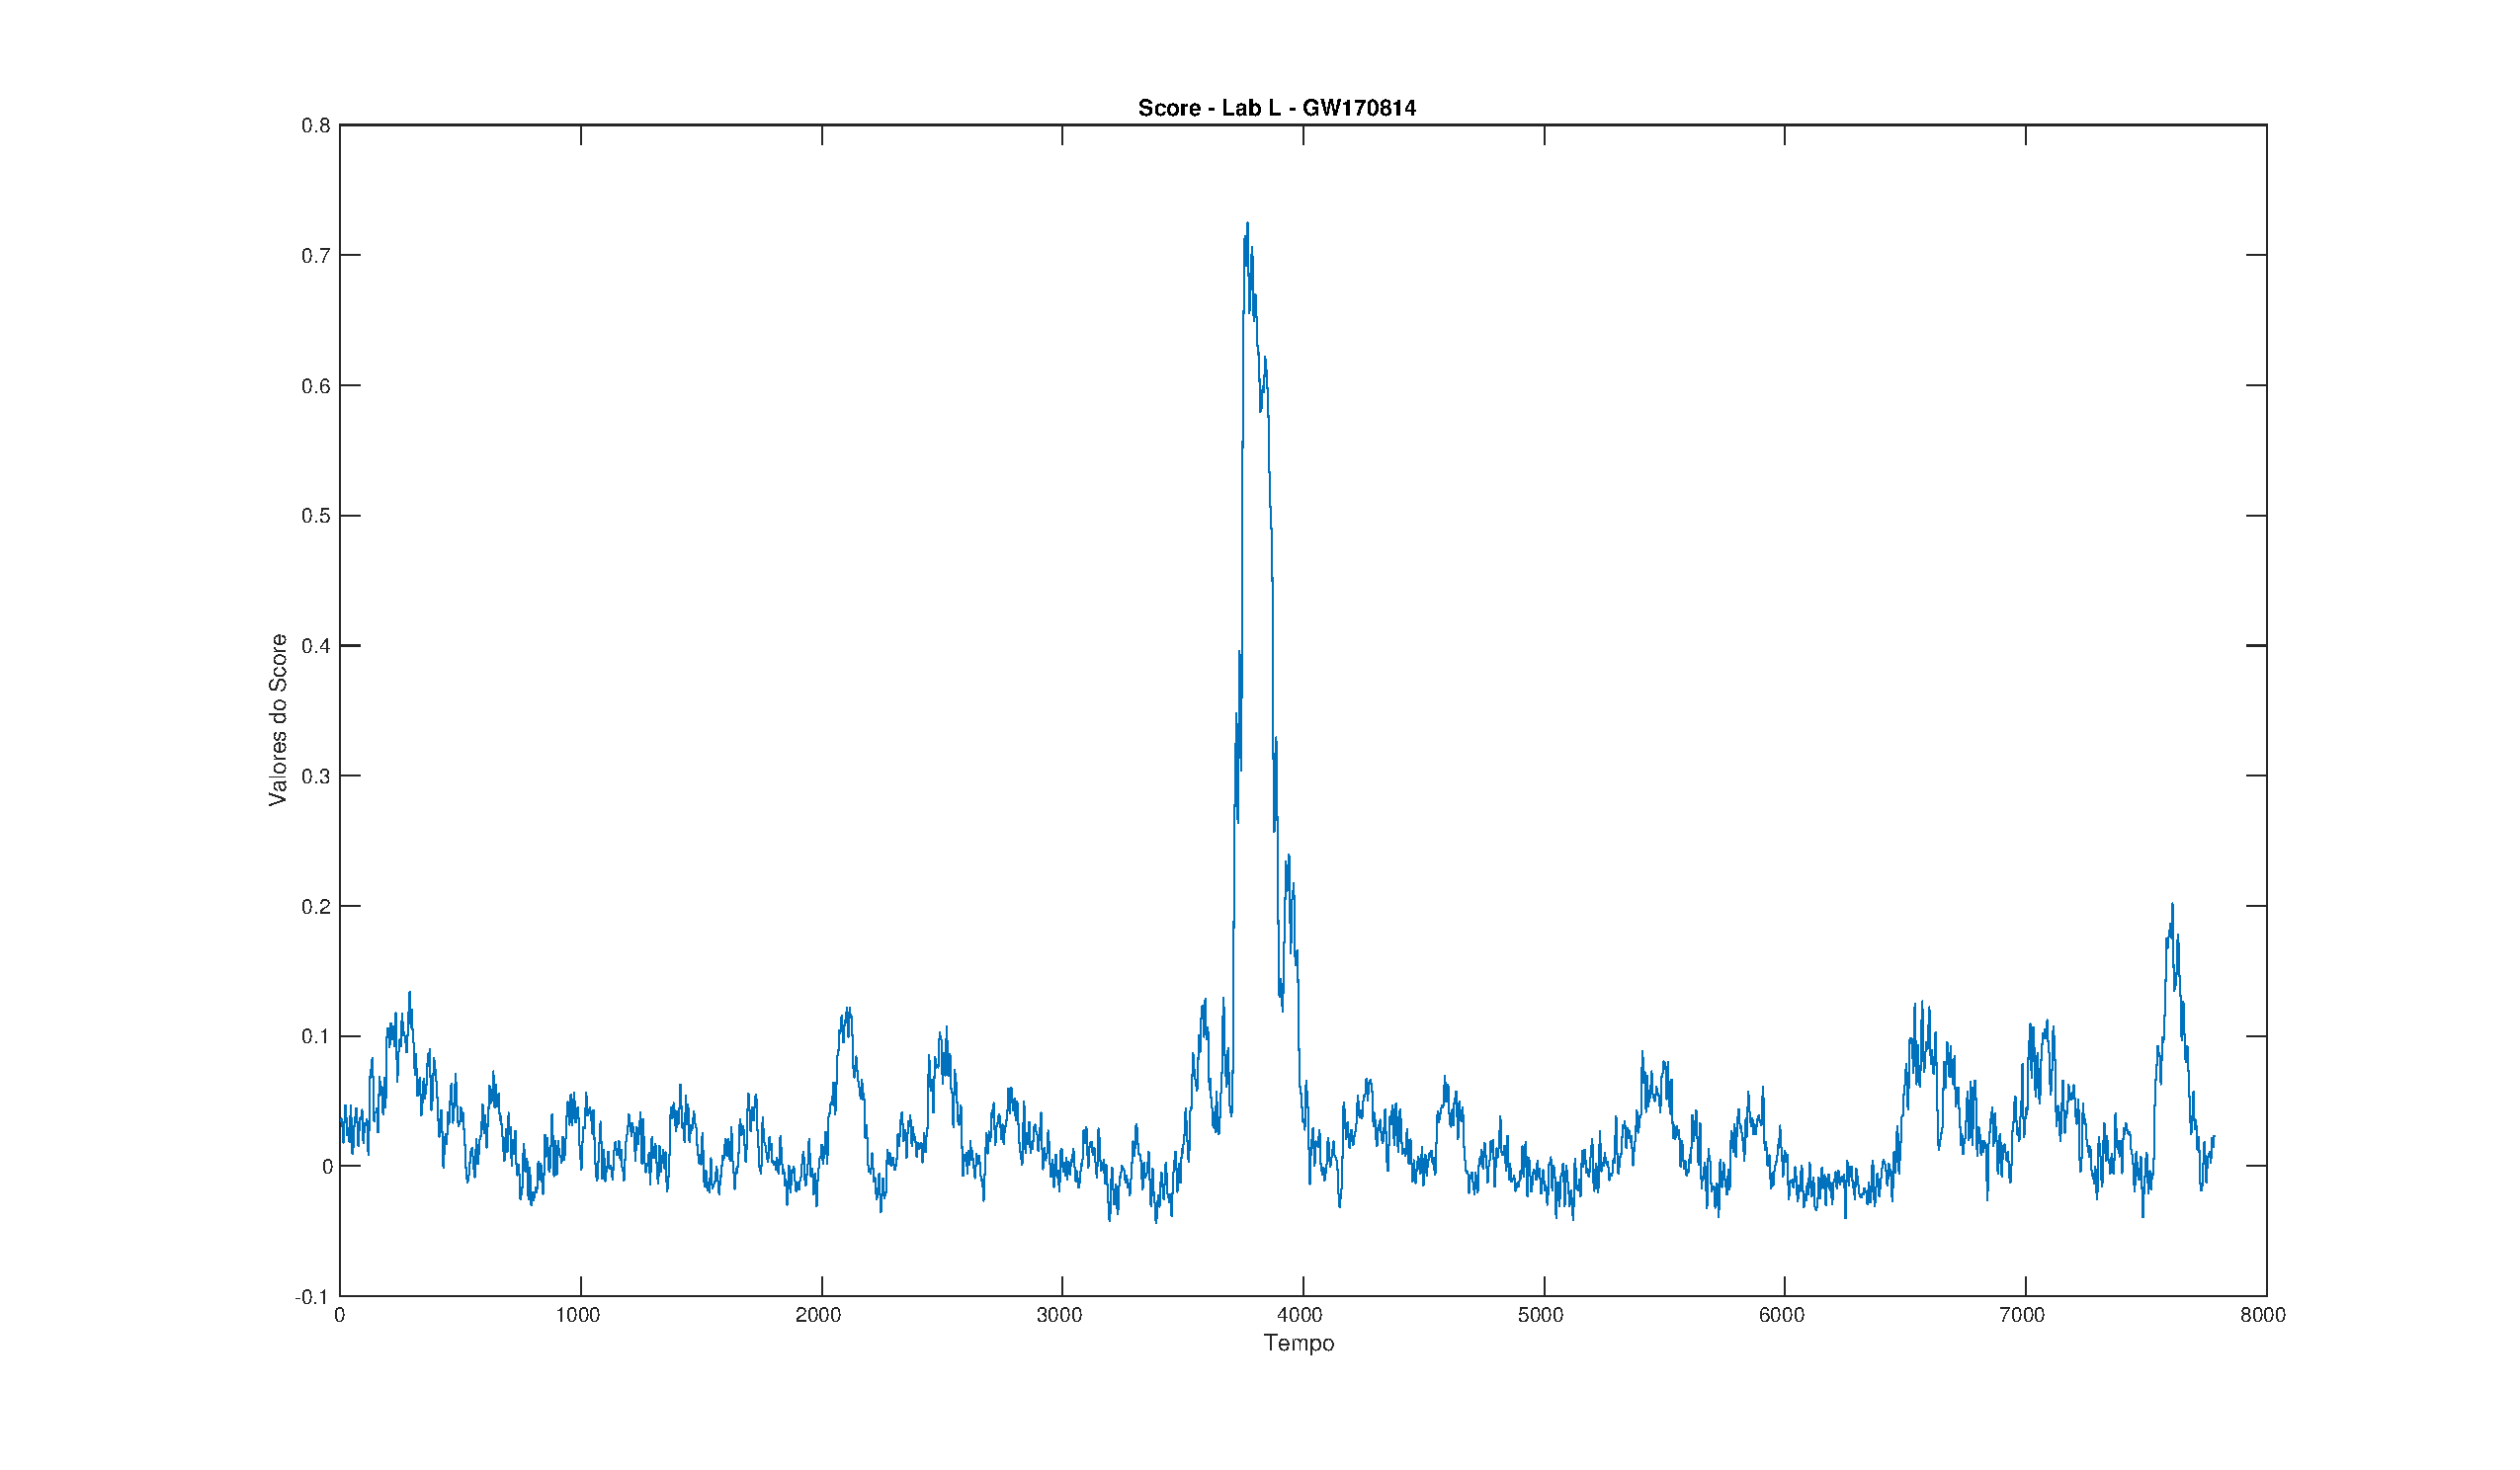
\includegraphics[width=0.5\textwidth]{figuras/GW170814_LabL.eps}}
     \subfigure[Coincidência entre os dois scores]{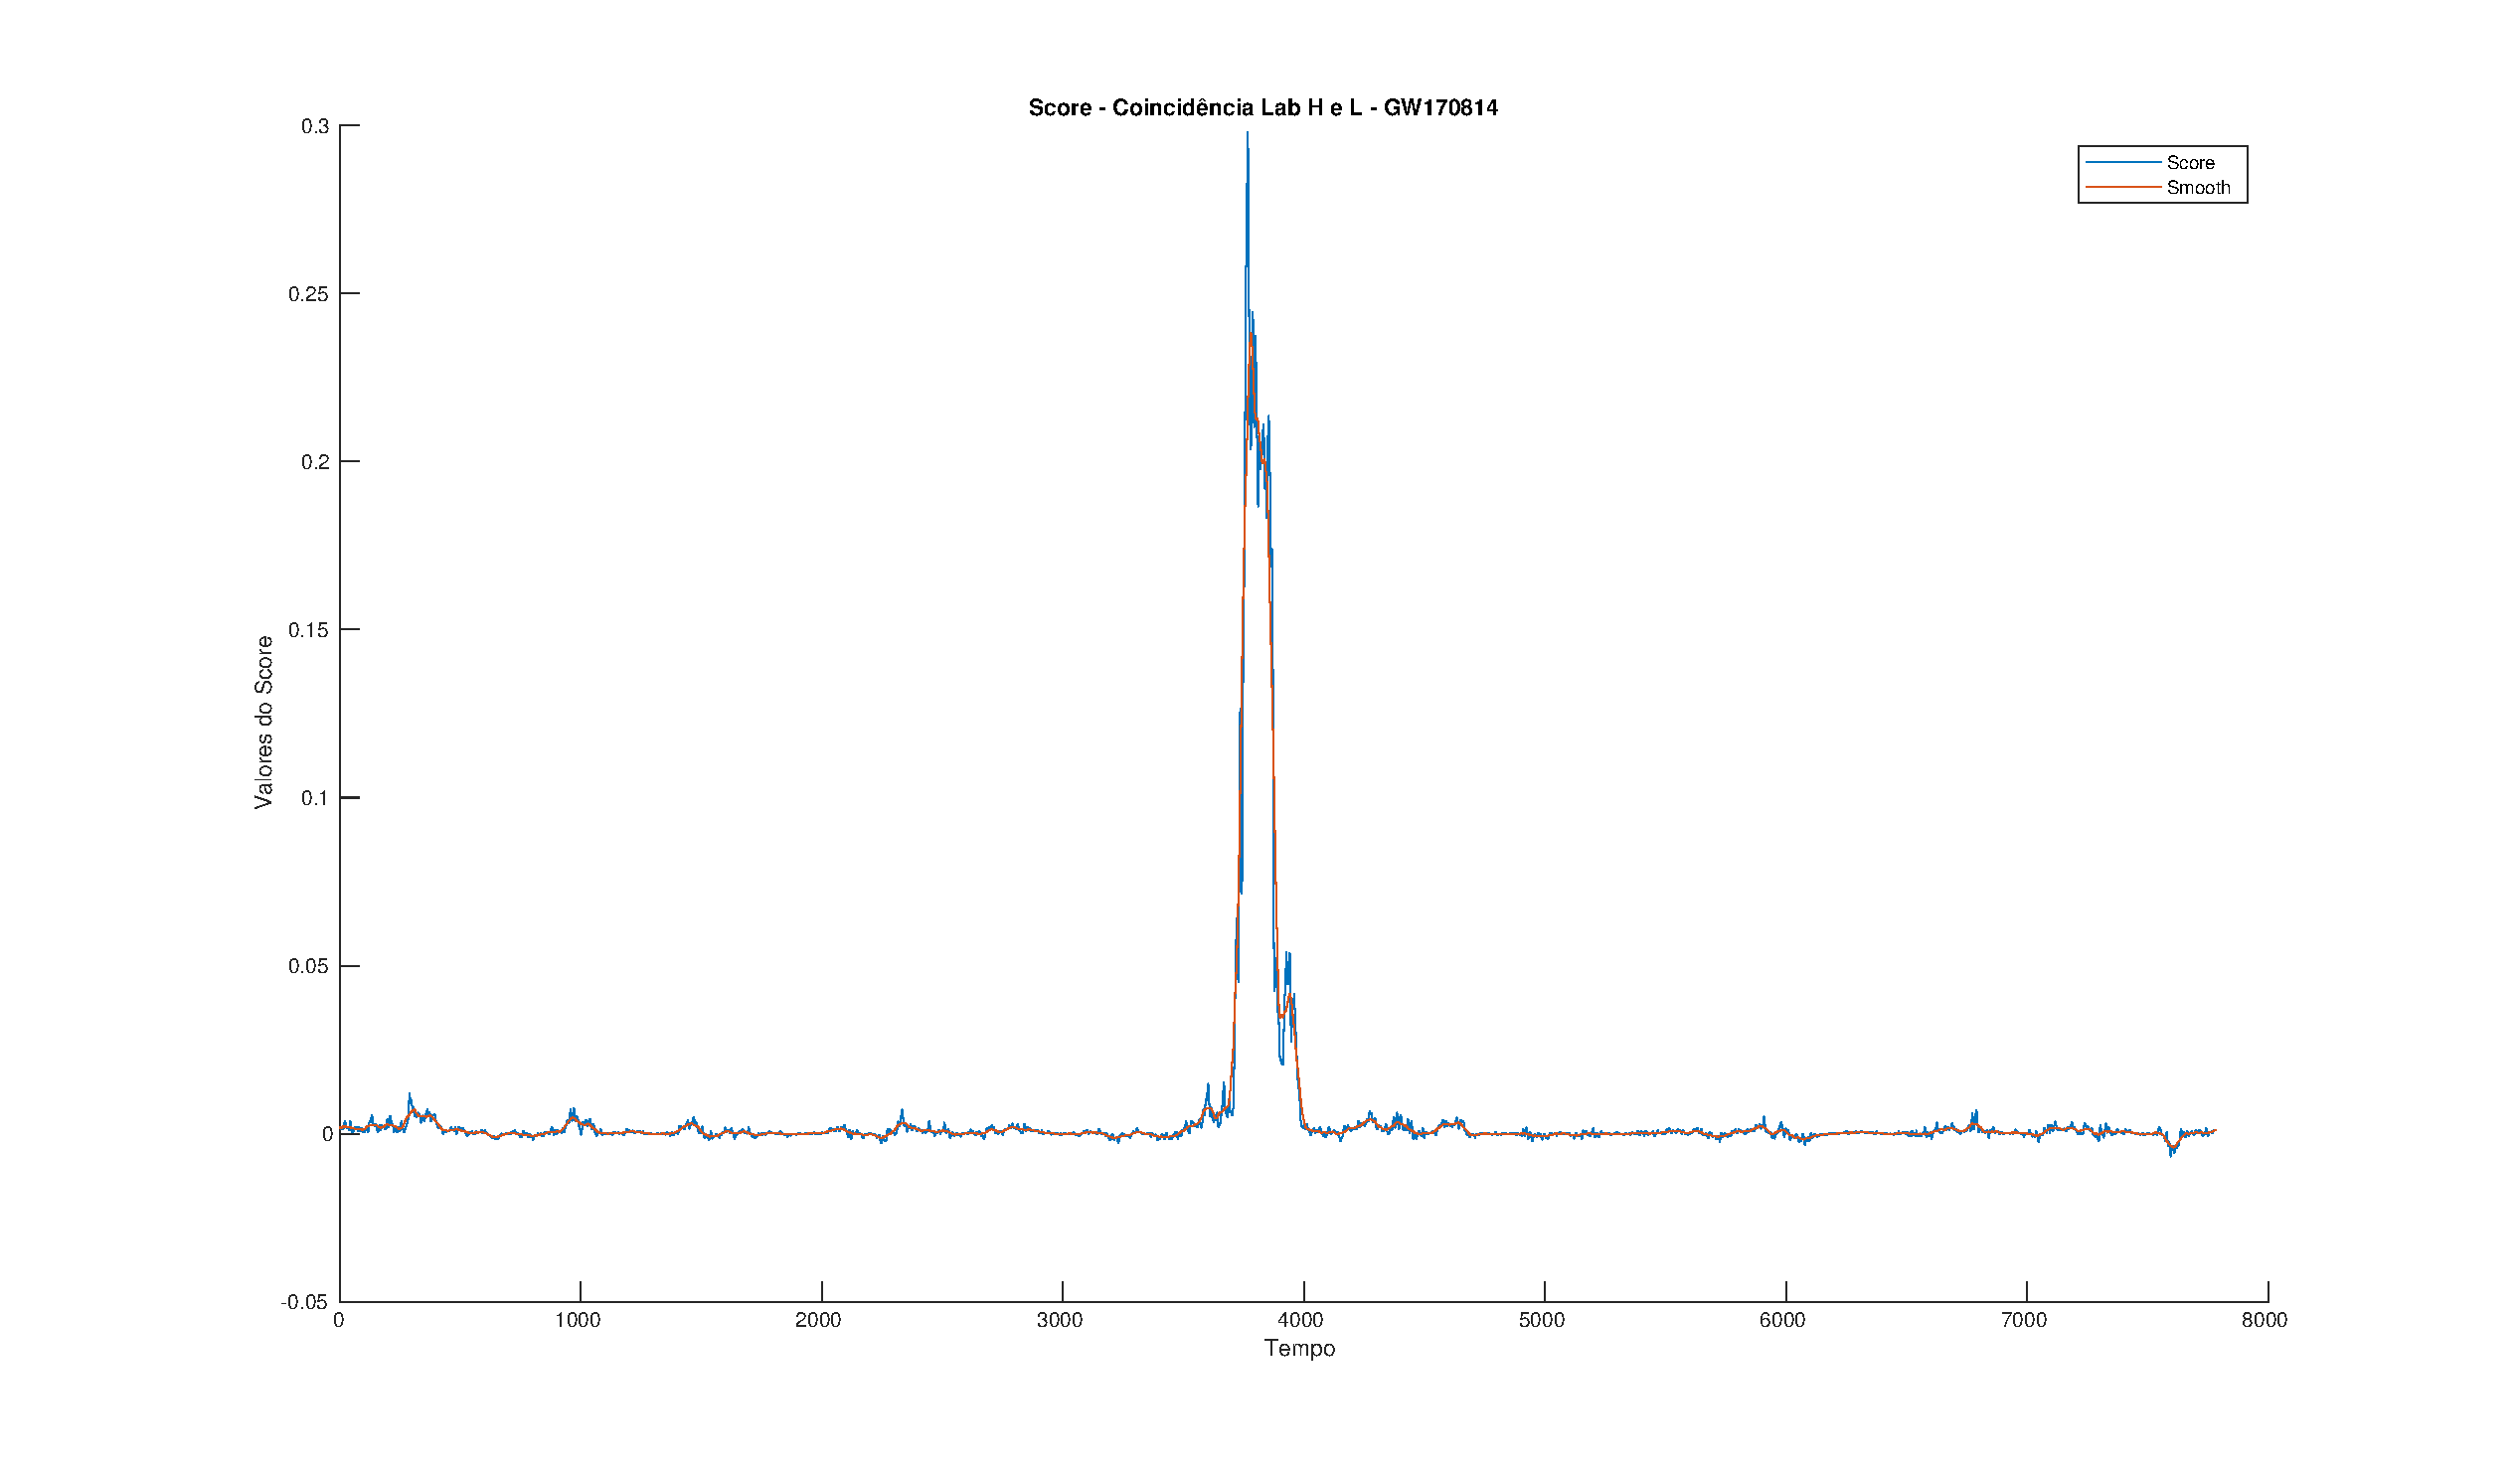
\includegraphics[width=1.0\textwidth]{figuras/GW170814_LabHL.eps}}
     \caption{Score da onda gravitacional GW170814}
 \end{figure}
 
\section{Score da onda gravitacional GW170823}
\begin{figure}[H]
     \subfigure[Score gerado para o laboratório H]{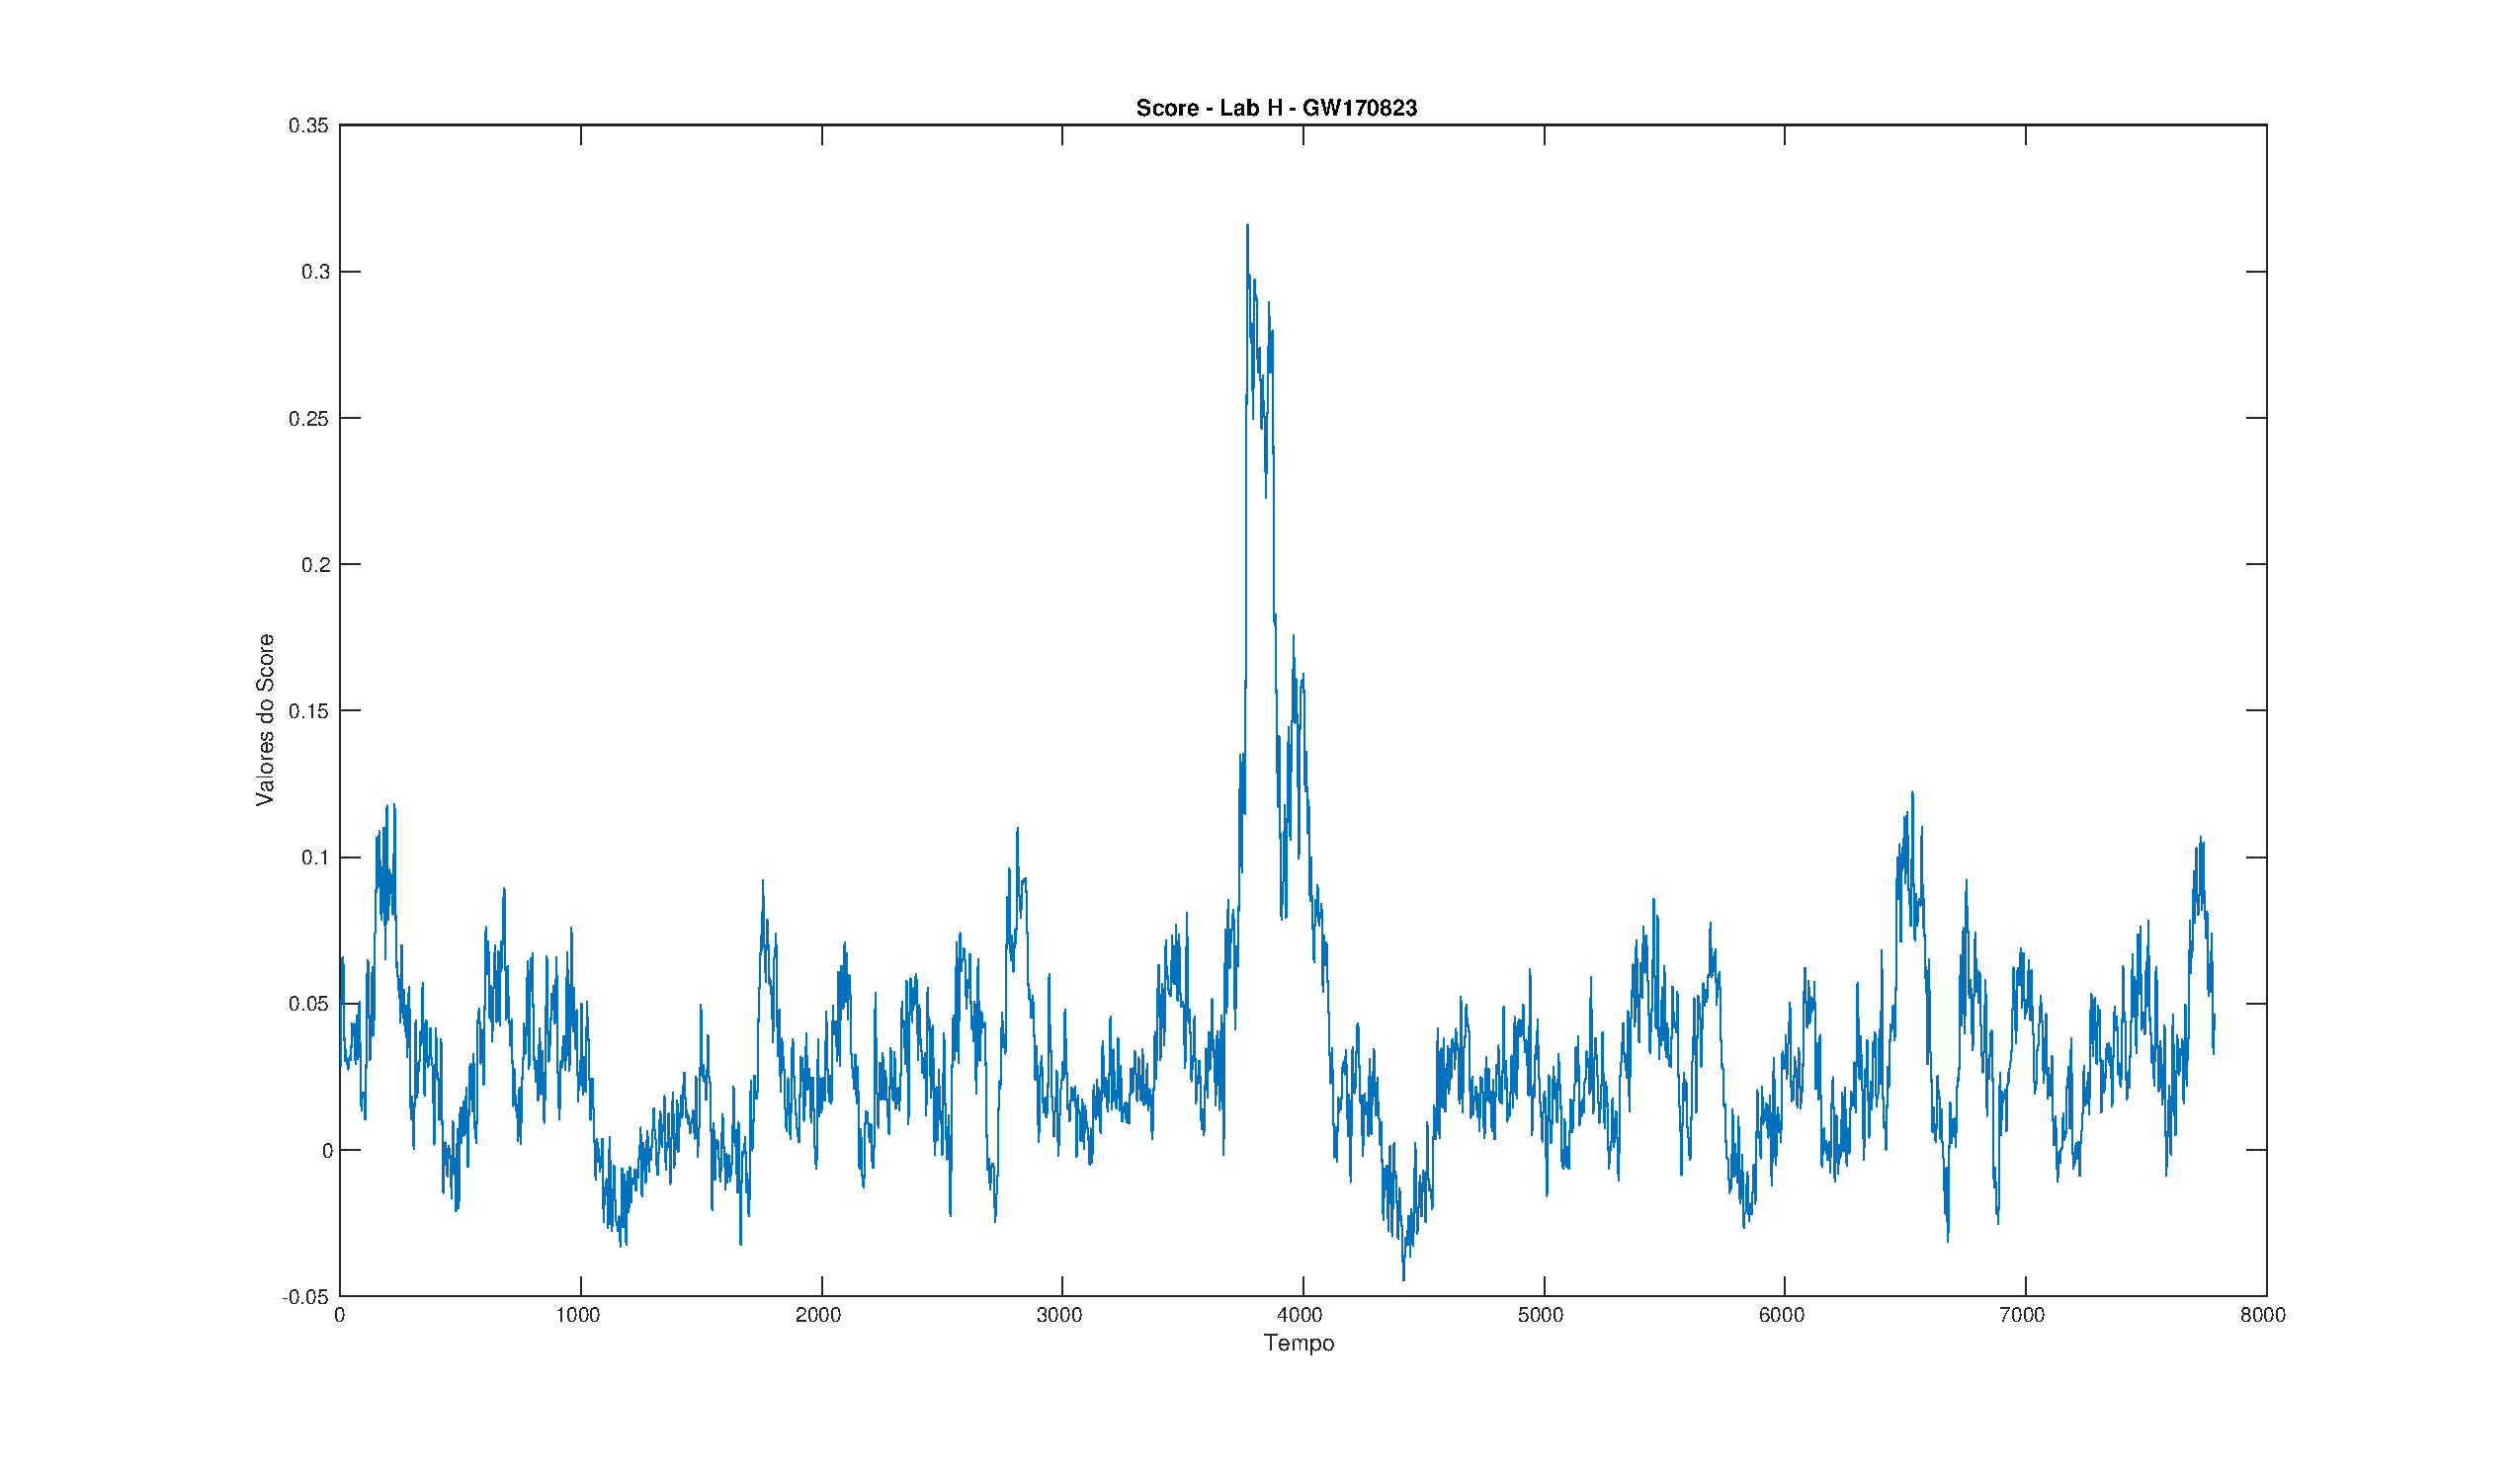
\includegraphics[width=0.5\textwidth]{figuras/GW170823_LabH.eps}}
     \subfigure[Score gerado para o laboratório L]{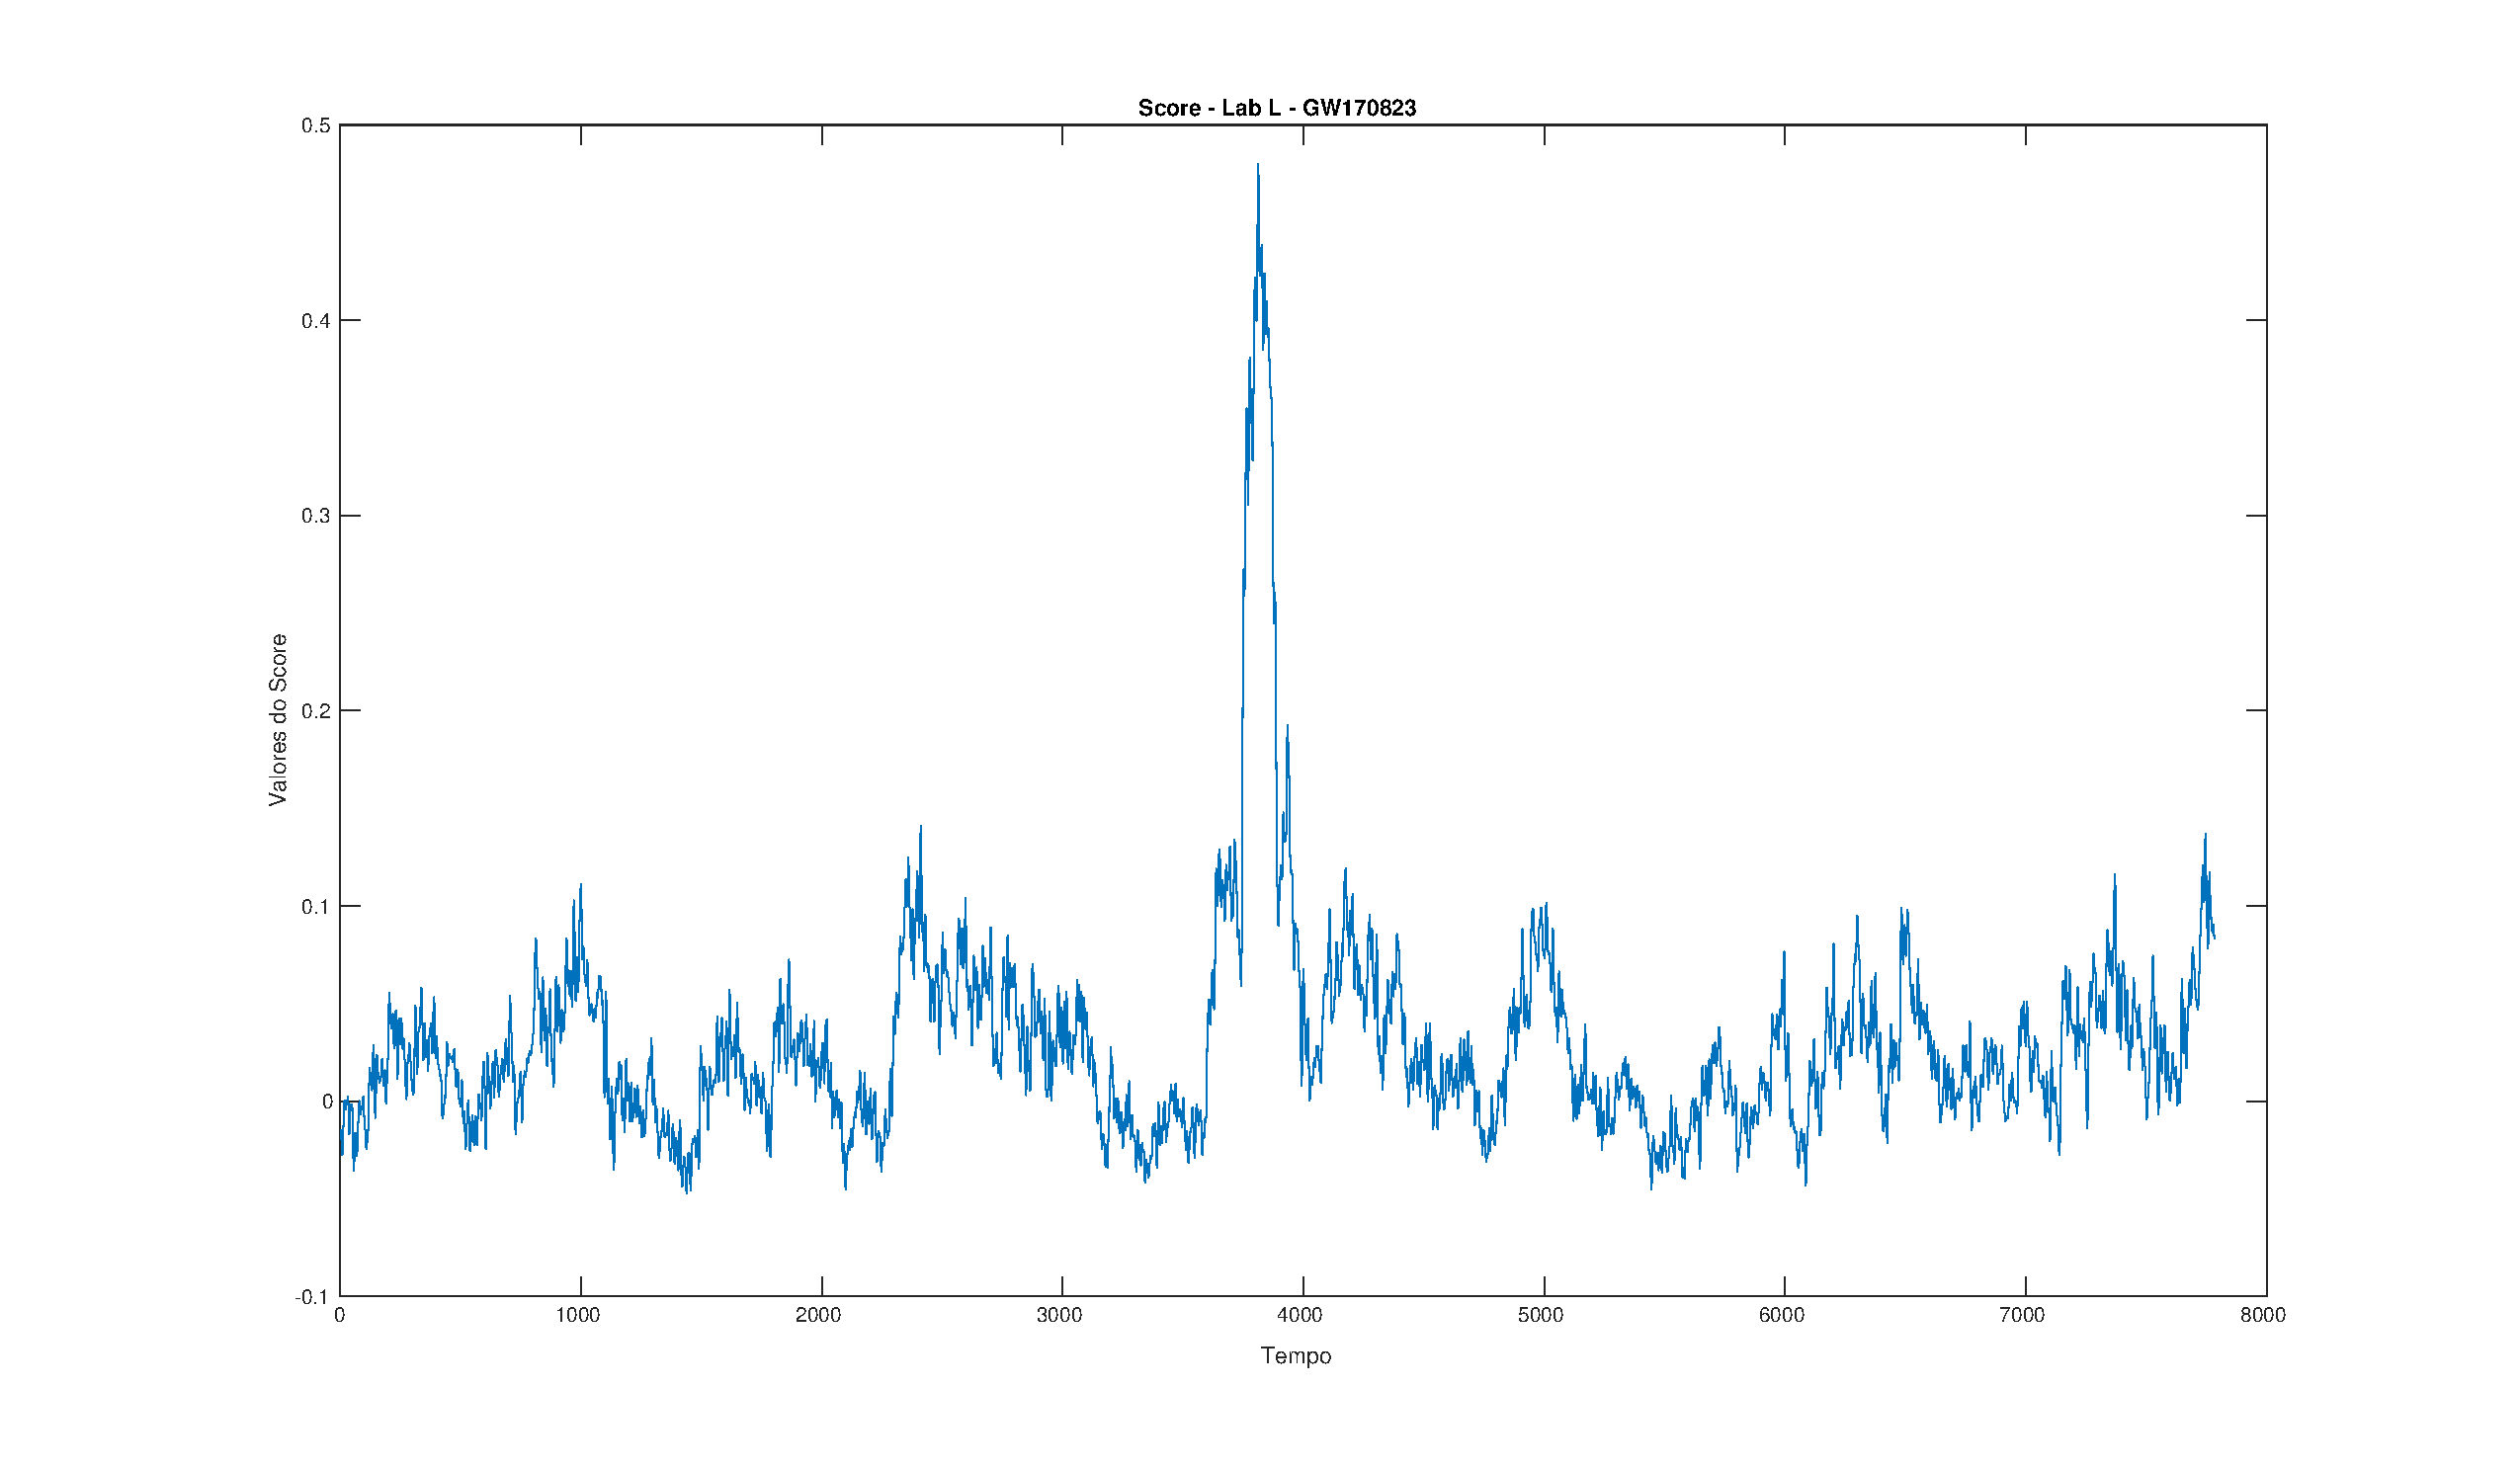
\includegraphics[width=0.5\textwidth]{figuras/GW170823_LabL.eps}}
     \subfigure[Coincidência entre os dois scores]{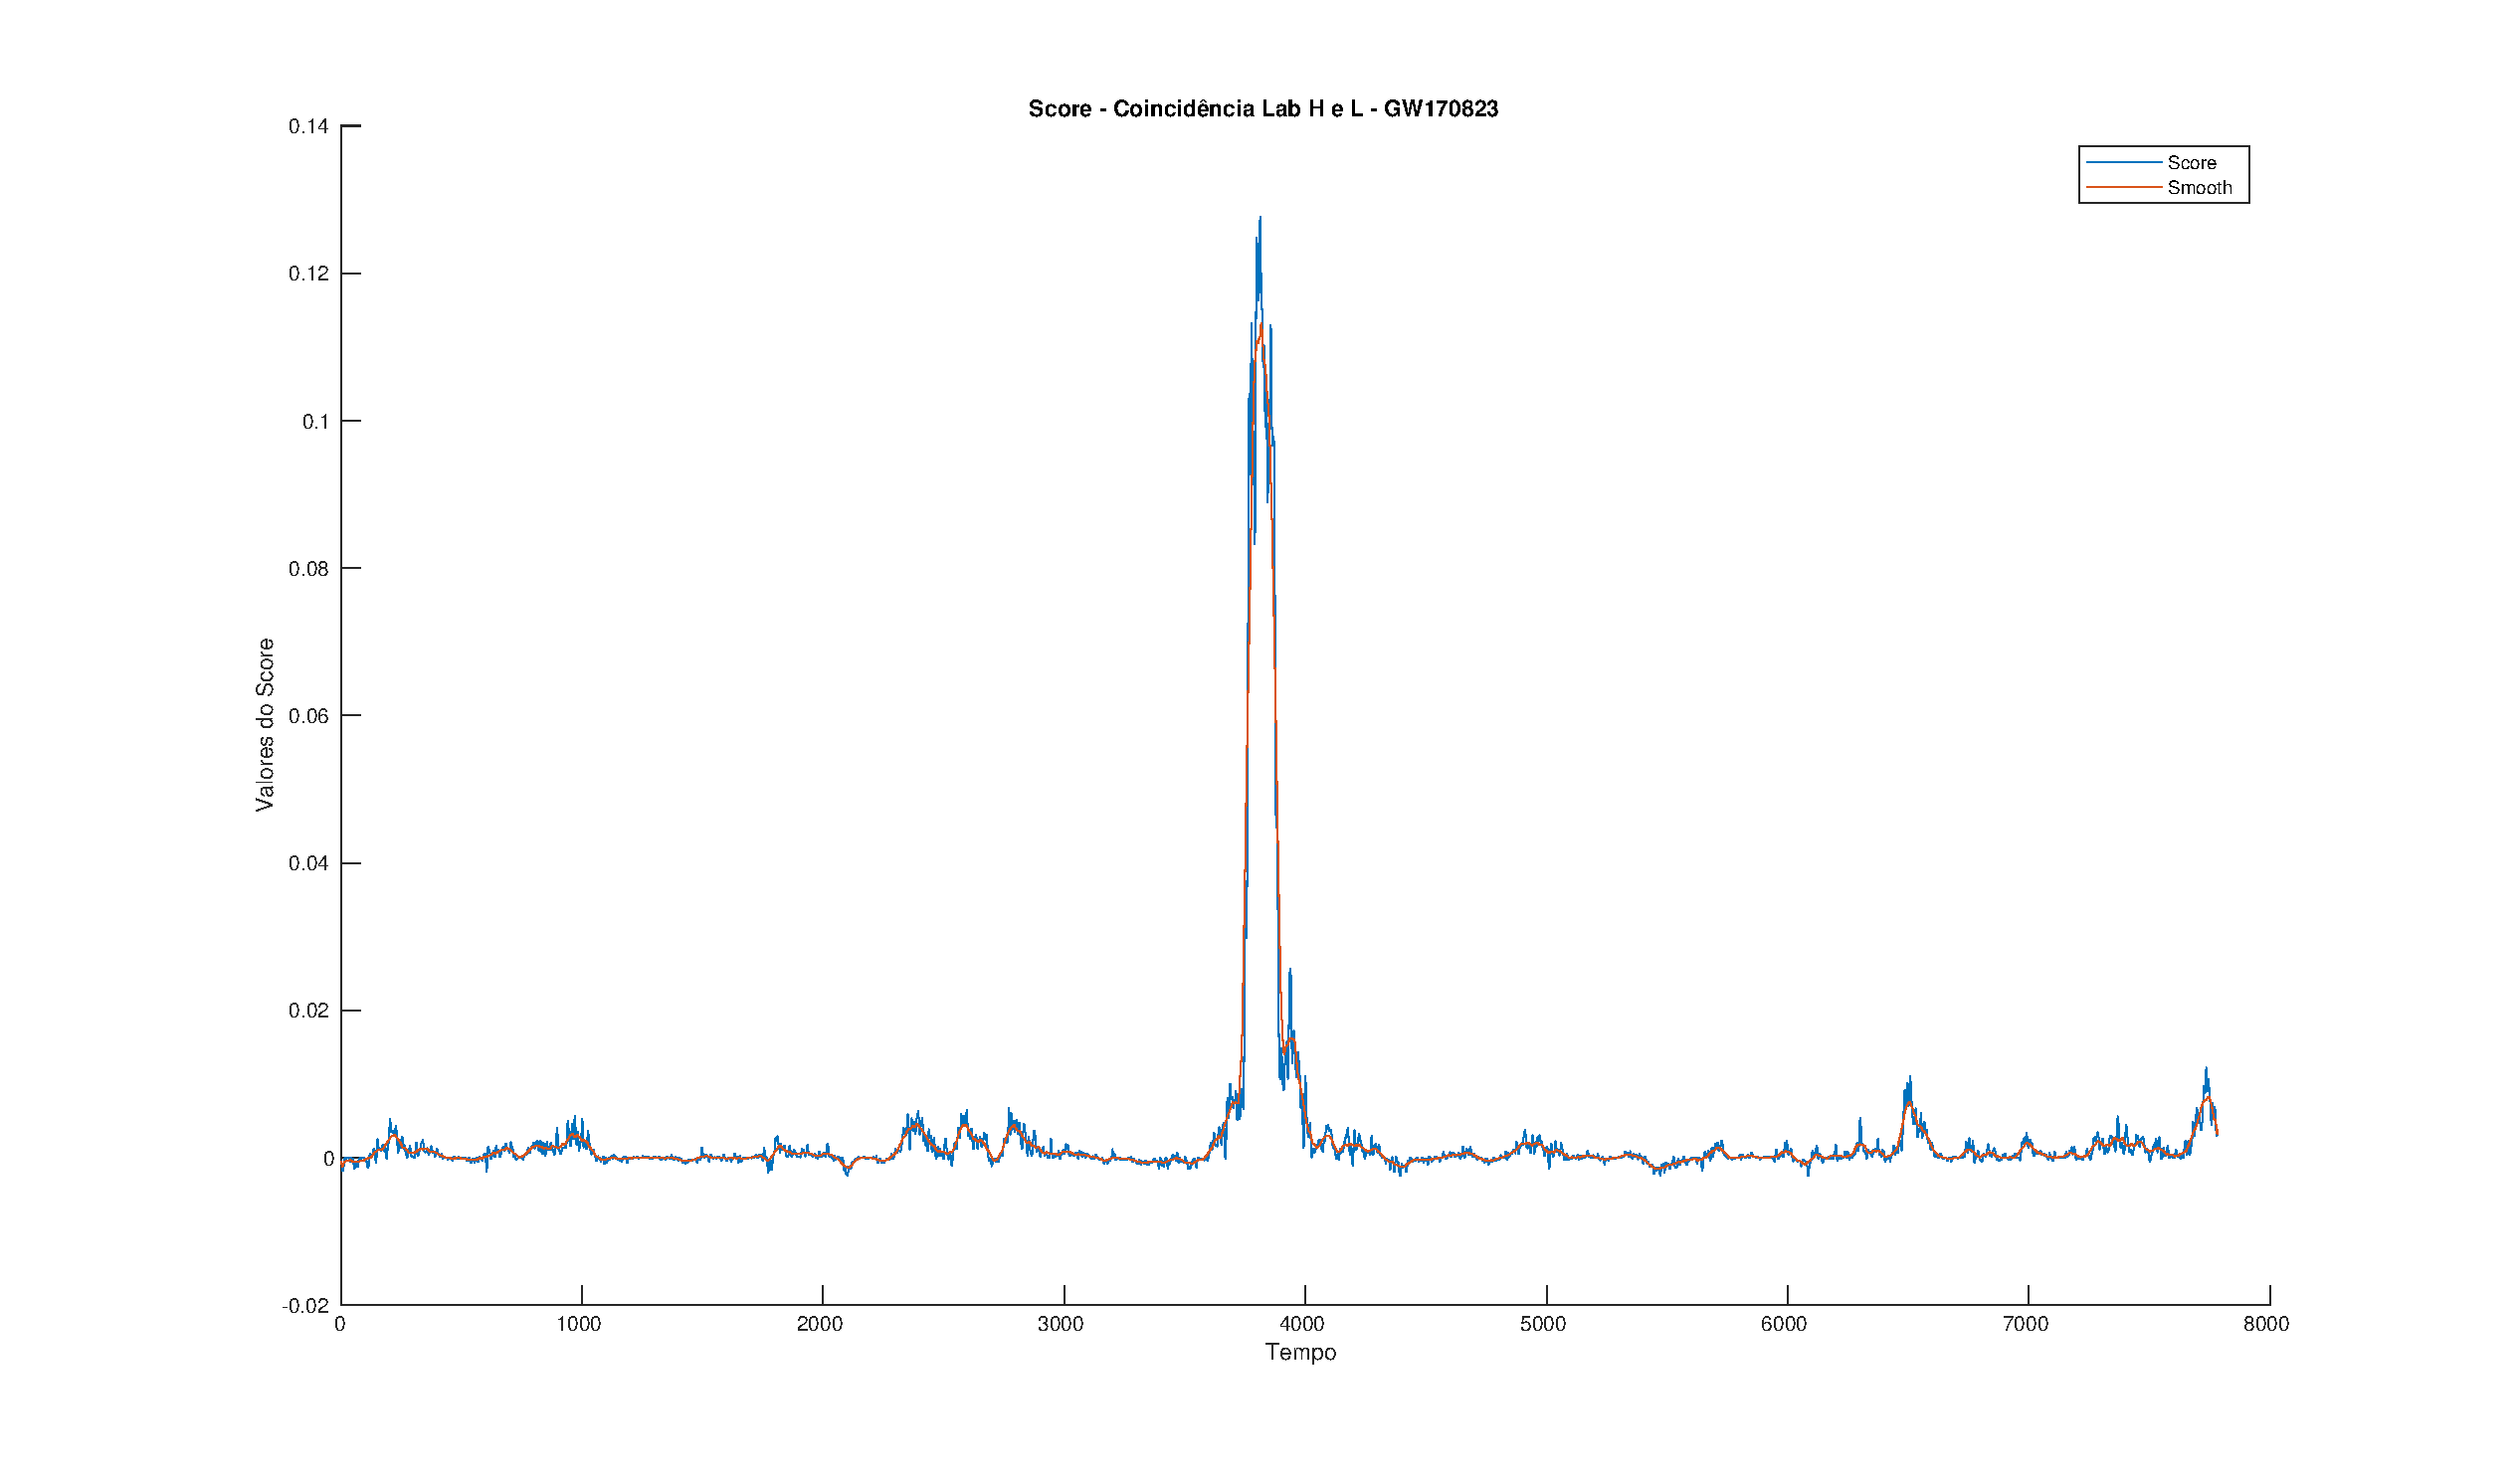
\includegraphics[width=1.0\textwidth]{figuras/GW170823_LabHL.eps}}
     \caption{Score da onda gravitacional GW170823}
 \end{figure}